\documentclass[
    a4paper,
    titlepage,
    headinclude,
    %footinclude,
    BCOR5mm,
    numbers=noenddot,
    cleardoublepage=empty,
    tablecaptionabove,
    fontsize=11pt,
    open=right,
    twoside,
    english,
    %draft
    %final
]{scrbook}
\usepackage[T1]{fontenc}
\usepackage[utf8]{inputenc}
\usepackage[italian,main=english]{babel}

%\usepackage[eulerchapternumbers,subfig,beramono,eulermath,pdfspacing]{classicthesis}
%\usepackage[eulerchapternumbers,subfig,eulermath,pdfspacing]{classicthesis}
%\usepackage{arsclassica}


% -- For drafting ------------
%\usepackage{lineno}
%\usepackage{setspace}
%\renewcommand{\baselinestretch}{2.0}
%\usepackage{showkeys}
% ----------------------------


% TODO Setup typography (fonts, mparhack, microtype...)
%\input{config/typographyConfig}
\renewcommand{\sfdefault}{iwona}

% Define some useful colors
\usepackage[dvipsnames]{xcolor}

% Define some colors
\definecolor{webgreen}{rgb}{0,.5,0}
\definecolor{webbrown}{rgb}{.6,0,0}
\definecolor{Maroon}{cmyk}{0, 0.87, 0.68, 0.32}
\definecolor{RoyalBlue}{cmyk}{1, 0.50, 0, 0}

% Setup plots
\usepackage{pgfplots}
\pgfplotsset{compat=newest}
\pgfplotsset{
    grid = major,
    major grid style={densely dotted},
    enlargelimits=.05,
    width = .75\textwidth
}
\usepgfplotslibrary{
    fillbetween,
    colormaps,
    units
}

\usepgfplotslibrary{external}
\tikzexternalize%[prefix=TikZ_pictures/]

\usepackage{tikz}
\usepackage{tikz-uml} % For UML diagrams

\usetikzlibrary{
    calc,
    shapes
}
\tikzset{>=stealth,}
\pgfplotsset{
    phase_plot/.style={%
        yticklabel style={sloped like y axis},%
        xlabel = {Mass of the final-state $\Ppiplus\Ppiminus$ system $[\si{\giga\electronvolt/\square\c}]$},
        %x unit = {\si{\giga\electronvolt/\square\c}},
        ylabel = {Dynamic-shape phase $[\si{deg}]$},
        %y unit = {\si{deg}}
    },
    amplitude_plot/.style={%
        yticklabel style={sloped like y axis},%
        xlabel = {Mass of the final-state $\Ppiplus\Ppiminus$ system $[\si{\giga\electronvolt/\square\c}]$},
        %x unit = {\si{\giga\electronvolt/\square\c}},
        ylabel = {Dynamic-shape magnitude $[\si{1\per(\giga\electronvolt/\square\c)^2}]$},
        %y unit = {\si{1\per(\giga\electronvolt/\square\c)^{-2}}}, % misaligns the plots
    },
    fit/.style={%
        mark options={%
            mark size=.75,%
            color=Maroon,%
            mark=*%
        },%
        ybar interval,%
        color=ForestGreen,%
        fill=LimeGreen,%
        fill opacity=.3,%
        % -- error bars --------
        error bars/y dir=both,%
        error bars/y explicit,%
        error bars/error bar style={color=Maroon},%
    },%
    guess/.style={%
        line width=.6,
        color=blue,
        mark=none,
        %mark options={%
        %    mark size=.75,
        %    mark=square*%
        %},%
    },%
    dalitz_plot/.style={%
        yticklabel pos=right,
        view={0}{90},%
        xlabel = {$m_{\Ppiplus\Ppiminus}^2$ $[\si{\giga\electronvolt^2\!/\c^4}]$},%
        ylabel = {$m_{\Ppiplus\Ppiminus}^2$ $[\si{\giga\electronvolt^2\!/\c^4}]$},%
        %x unit = {\si{\giga\electronvolt^2\!/\c^4}},%
        %y unit = {\si{\giga\electronvolt^2\!/\c^4}},%
        %colormap/viridis high res,%
        %colormap/winter,%
        colorbar left=true,%
        colorbar left/.append style={%
            yticklabel style={sloped like x axis},%
        },%
        %axis equal,%
    },%
    dalitz/.style={%
        scatter,%
        scatter src=z,%
        only marks,%
        mark options={%
            mark=square*,%
            mark size=1.1,%
        }%
    }%
}

\usepackage{subfig}
\usepackage{rotating}
\usepackage{booktabs}
% For the background coffee stain in the acknowledgements page.
\usepackage{eso-pic}

% Setup units
\usepackage{siunitx}

\sisetup{
%	range-phrase=$-$,
	separate-uncertainty,
%	input-decimal-marker={.},
	output-decimal-marker={.},
	exponent-product = \cdot,
}

% Additional units

\usepackage{eurosym}
\DeclareSIUnit{\EUR}{\text{\euro{}}}
\DeclareSIUnit{\c}{\text{c}}

% Setup math
\usepackage{amsmath}

% For \ltrans
\usepackage{leftidx}

% Load constants
% Some useful math constants

% Euler number
\newcommand{\eu}{\ensuremath{\mathrm{e}}}
% Imaginary unit
\newcommand{\iu}{\ensuremath{\mathrm{i}}}

% Load delimiters
% Delimiters

% Among other tools, define DeclarePairedDelimiter
\usepackage{mathtools}

% Absolute value |-|
\DeclarePairedDelimiter{\abs}{\lvert}{\rvert}
% Norm ||-||
\DeclarePairedDelimiter{\norm}{\lVert}{\rVert}

% For \Set, \bra, \ket and so on
\usepackage{braket}

% Custom parentheses
\DeclarePairedDelimiter{\roundB}{(}{)}
\DeclarePairedDelimiter{\squareB}{[}{]}
\DeclarePairedDelimiter{\curlyB}{\{}{\}}

% Mean <.>
\DeclarePairedDelimiter{\mean}{\langle}{\rangle}

% Load numbersets
% Numbersets

% To enable \mathbb
% Also enables \Cap, \Box, \Diamond and so on
\usepackage{amssymb} % loads amsfonts

% Numbersets ------------------------
\newcommand{\numberset}[1]{\ensuremath{\mathbb{#1}}}
\newcommand{\N}{\numberset{N}}
\newcommand{\Z}{\numberset{Z}}
\newcommand{\Q}{\numberset{Q}}
\newcommand{\R}{\numberset{R}}
\newcommand{\I}{\numberset{I}}
\newcommand{\C}{\numberset{C}}
% Euclidean space
\newcommand{\E}{\numberset{E}}
% -----------------------------------

% Empty set
\newcommand{\0}{\ensuremath{\varnothing}}
% Cartesian product
\newcommand{\x}{\ensuremath{\times}}

% Load operators
% Operators

% Differential operators ------------
\newcommand{\de}{\mathop{}\!\textup{$\partial$}}
\newcommand{\uD}{\mathop{}\!\textup{$\Delta$}}
\newcommand{\ud}{\mathop{}\!\textup{d}}
\newcommand{\V}{\mathop{}\!\nabla}
\newcommand{\VV}{\ensuremath{\V^2}}
% D'Alembert operator
\newcommand{\dal}{\ensuremath{\mathop{}\!\Box}}
% -----------------------------------

% Algebra ---------------------------
\DeclareMathOperator{\tr}{tr}
\DeclareMathOperator{\diag}{diag}
% -----------------------------------

% Statistics ------------------------
\DeclareMathOperator{\erf}{erf}
\DeclareMathOperator{\cov}{cov}
% -----------------------------------


% Vectors
\usepackage{bm}
\renewcommand{\vec}[1]{\ensuremath{\mathbf{{#1}}}}

\newcommand{\A}{\ensuremath{\mathcal{A}}}
\newcommand{\Intensity}{\ensuremath{\mathcal{I}}}
\newcommand{\package}[1]{\textsf{#1}}
\newcommand{\ROOT}{{\footnotesize{\package{ROOT}}}}
\newcommand{\MINUIT}{{\footnotesize{\package{MINUIT}}}}
\newcommand{\cpp}[1][]{{\footnotesize{C++\ifthenelse{\equal{#1}{}}{}{#1}}}}
\newcommand{\eg}{e.g.}
\newcommand{\ie}{i.e.}

\newcommand{\collaboration}[1]{\textsc{#1}}
\newcommand{\cleo}{\collaboration{cleo}}
\newcommand{\focus}{\collaboration{focus}}

% Wrappers for the acronyms
% No plurals should be needed for packages
\newcommand{\pac}[1]{\package{\ac{#1}}}
\newcommand{\pacl}[1]{\package{\acl{#1}}}
\newcommand{\pacs}[1]{\package{\acs{#1}}}

% Setup listings
\usepackage[
    final
]{listings}
\lstset{
    language={[11]C++},%
    basicstyle=\ttfamily,%
    tabsize=4,%
    keywordstyle=\color{blue!50!black}\fontseries{b}\selectfont,%
    morekeywords={
        BreitWigner,%
        DataAccessor,%
        DataIterator,%
        DataPartition,%
        DataPoint,%
        DecayChannel,%
        DecayingParticle,%
        FinalStateParticle,%
        Flatte,%
        FlatteChannel,%
        HelicityFormalism,%
        MassBin,%
        MassShape,%
        MassShapeWithNominalMass,%
        Model,%
        Parameter,%
        Particle,%
        ParticleCombination,%
        ParticleFactory,%
        PoleMass,%
        PositiveRealParameter,%
        RealCachedValue,%
        RelativisticBreitWigner,%
        StaticDataAccessor,%
        ZemachFormalism,%
        shared_ptr,%
        unique_ptr,%
        vector,%
    },
    keywords=[2]{std, yap},% namespaces
    keywordstyle=[3]{\color{green!60!blue}\fontseries{b}\selectfont},%
    keywords=[3]{make_shared, make_unique, static_pointer_cast, complex, polar},% std-functions
    keywordstyle=[2]{\color{green!60!red}\fontseries{b}\selectfont},%
    keywords=[4]{calculate, addParameter, free_amplitude, setFinalState, lock, addInitialState, quantumNumbers, rad, addWeakDecay, addStrongDecay, create, to, read_pdl_file, add},% yap functions
    keywordstyle=[4]{\color{green!60!red}\fontseries{b}\selectfont},%
    commentstyle=\color{darkgray!80},%
    stringstyle=\color{orange!50!black},%
    frame=l,%
    numbers=left,%
    stepnumber=5,%
    numberstyle=\tiny\color{black!80},%
    escapeinside={£!}{!£},%
    %backgroundcolor=\color{cyan!10},%
}



% Setup index
% COnfiguration file for the index

\usepackage{makeidx}
\usepackage{multicol}

% enable generation of index via '\printindex' command in the document environment
\makeindex

%%
\let\orgtheindex\theindex
\let\orgendtheindex\endtheindex
\def\theindex{%
	\def\twocolumn{\begin{multicols}{2}}%
	\def\onecolumn{}%
	\clearpage
	\orgtheindex
}
\def\endtheindex{%
	\end{multicols}%
	\orgendtheindex
}
%%%%%%%%%%%%%%%%%%%%%%%%%%%

% Setup bibliography
% Setup bibliography
\usepackage[
	backend=biber,
]{biblatex}
\usepackage{csquotes}
\addbibresource{backmatter/bibliography.bib}


% Define abstract environment for *book class
% Define the abstract environment in a book (or scrbook) documentclass
%\usepackage{fancyhdr}
%\newcommand{\fncyblank}{\fancyhf{}}
\newenvironment{abstract}%
{\cleardoublepage\thispagestyle{empty}\null\vfill\begin{center}%
\bfseries\abstractname\end{center}}%
{\vfill\null}

% Define acknowledgements environment
% XXX Load _after_ abstractConfig.tex!!
% Define the acknowledgements environment in a book (or scrbook) documentclass

% These are already loaded/defined in abstractConfig.tex
%\usepackage{fancyhdr}
%\newcommand{\fncyblank}{\fancyhf{}}

\newenvironment{acknowledgements}%
{\cleardoublepage\fncyblank\null\vfill\begin{center}%
\bfseries{Acknowledgements}\end{center}}%
{\vfill\null}


% Setup hyperref
% Setup hyperref
\usepackage{hyperref}
\hypersetup{
    %draft,
    final,
    %colorlinks=false,
    colorlinks=true,
    linktocpage=true,
    pdfstartpage=3,
    pdfstartview=FitV,
    breaklinks=true,
    pdfpagemode=UseNone,
    pageanchor=true,
    pdfpagemode=UseOutlines,%
    plainpages=false,
    bookmarksnumbered,
    bookmarksopen=true,
    bookmarksopenlevel=1,%
    hypertexnames=true,
    pdfhighlight=/O,
    urlcolor=webbrown,
    linkcolor=RoyalBlue,
    citecolor=webgreen,
%   pagecolor=RoyalBlue,%
}

% Setup acronyms
% XXX Load it _after_ hyperref, babel, polyglossia, inputenc and fontenc
% For acronyms (and glossaries)
\usepackage[
	makeindex,% use this to make gloxary
	acronym,%
	nomain,% suppress the main (default) glossary
	hyperfirst=false, % no hyperlink at first use of acronym
	toc,% add voice in toc
]{glossaries} % XXX Load it _after_ hyperref, babel, polyglossia, inputenc and fontenc

\usepackage{relsize} % defines \textsmaller{} used by the following style
\setacronymstyle{long-sm-short}

\makenoidxglossaries


% Define acronyms
\newacronym{cuda}{CUDA}{Compute Unified Device Architecture}


\usepackage{caption}

% Add this package to draw molecules (needed for the caffeine!)
\usepackage{chemfig}
% Change atom font in molecule figures
\renewcommand*\printatom[1]{\ensuremath{\mathsf{#1}}}

\usepackage[
%    notitalic, % particle names are upright
]{hepnames}
\newcommand{\Pfnez}{\HepParticleResonanceFull{f}{0}{}{980}{}{}{}}
\newcommand{\Pfofzz}{\HepParticleResonanceFull{f}{0}{}{1500}{}{}{}}
\newcommand{\Pfotsz}{\HepParticleResonanceFull{f}{0}{}{1370}{}{}{}}
\newcommand{\Psigma}{\HepParticleResonanceFull{f}{0}{}{500}{}{}{}}
\usepackage{qrcode}

\title{Development of software for model-independent analysis of multi-body hadronic decays}
\subtitle{}
\author{
  \input{AUTHORS}
}
\date{}

\begin{document}
%\linenumbers


%----------------------------------------------------------------------------------------
% FRONTMATTER
%
\frontmatter
\phantomsection
\pdfbookmark[0]{Title}{chap:title}
    \maketitle
    \thispagestyle{empty}

    \cleardoublepage
\phantomsection
\pdfbookmark[0]{Dedication}{chap:dedication}
    \thispagestyle{empty}
    \null\vspace{\stretch {1}}
        \begin{flushright}
                This is the Dedication.
        \end{flushright}
\vspace{\stretch{2}}\null


    \cleardoublepage
\phantomsection
\pdfbookmark[0]{\abstractname}{chap:abstract}
    \begin{abstract}
    Partial-wave analysis is currently the standard analysis technique in the study of hadronic heavy-meson decays.
    In this context, to find an explicit form of the decay amplitude, most analyses exploit the isobar model, which assumes that the decay of the parent particle proceeds through subsequent two-body decays involving well-defined intermediate states.
    The success of the isobar model in providing a good description of the decay depends on the assumptions about these intermediate states.


    Due to the availability of increasingly large experimental data sets, the systematic uncertainty introduced by partial or incorrect knowledge of the intermediate states dominate the statistical uncertainty.
    A possible extension of the current analysis techniques is the model-independent approach to partial-wave analysis:
    It exploits the increase of the experimental data samples to get rid of unjustified assumptions of the isobar model, as the properties of the isobars are extracted from the data itself.


    Because of the large experimental data sets and the large number of fit parameters, partial-wave analyses involve expensive calculations.
    This motivates the development of \pacs{yap}, a novel toolkit for partial-wave analysis.


    Here, after introducing the partial-wave-analysis formalism, I describe the main features of \pacs{yap} and present my \pacs{yap}-based implementation of a model-independent partial-wave-analysis fit utility.
    I also show the test fits I performed on several \acs{mc} data sets of $\PDplus\to\Ppiplus\Ppiminus\Ppiplus$ decays with increasing number of waves.
    The \acs{mc} data generated according to the fitted parameters correctly reproduce the fit source data.

\end{abstract}


    \cleardoublepage
\phantomsection
\pdfbookmark[0]{Acknowledgements}{chap:acknowledgements}
    %\chapter*{Aknowledgements}
%\phantomsection
%\addcontentsline{toc}{chapter}{Aknowledgements}


\begin{acknowledgements}
\dots{}

Last but not least I'd like to thank you, Caffeine, I would not have made it without you!

% Draw a Caffeine molecule
\setcrambond{2pt}{}{}
\setatomsep{2em}
\chemname{%
\chemfig{%
{\color{black!70}H_3C}-[:72]{\color{RoyalBlue}N}%
    *5(-%
	*6(-(={\color{Maroon}O})-{\color{RoyalBlue}N}(-{\color{black!70}CH_3})-(={\color{Maroon}O})-{\color{RoyalBlue}N}(-{\color{black!70}CH_3})-=)%
    --{\color{RoyalBlue}N}=-)}%
}{}

\end{acknowledgements}


    \cleardoublepage
\phantomsection
\pdfbookmark[0]{\contentsname}{chap:contents}
    \tableofcontents

%----------------------------------------------------------------------------------------
% MAINMATTER
%
\mainmatter

    \chapter{Introduction}

    The aim of this thesis is the description of \pac{yap}, a novel \ac{pwa} toolkit that I have contributed to develop.
    I also show the results of some model-independent fits performed using a self-developed piece of software relying on the external libraries \pac{yap} and \pac{bat}.

    \section{Physical motivation}

    Examples of usage:
    \begin{itemize}
        \item Searches for new states;
        \item Measuging resonance properties;
        \item $CP$ violation;
        \item B and D mixing;
        \item Resolving ambiguities.
    \end{itemize}

    \chapter{\texorpdfstring{\Acl{pwa}}{Partial-wave analysis}}
\label{chap:theory}

    \Ac{pwa}\index{partial-wave analysis} is a standard technique in scattering theory.
    It allows to write down the scattering probability amplitude in terms of Legendre polynomials, the eigenvectors of the angular momentum operator, each representing a partial\index{partial wave} wave~\cite[\S~11.2]{griffiths_intro_qm}.


    In this chapter, I will show how to apply the \ac{pwa} to heavy-meson decays to disentangle the various contributions to the decay amplitude.
    I will focus on the isobar decomposition of a spinless parent particle to three pseudo-scalar spinless daughter particles in the final state.
    This is the case of the $\PDplus\to\Ppiplus\Ppiminus\Ppiplus$ decay, to which I will refer throughout the whole thesis.


    In the last part of the chapter, I will briefly introduce the reader to the Dalitz plot, a particularly useful visualization tool in the \ac{pwa} of three-body particle decays.

    \section{Isobar decomposition}

    In quantum mechanics, the quantity that describes the distribution of the observed events in an experiment is the event intensity\index{intensity}, $\Intensity(\tau)$, $\tau$ being the phase-space coordinate of the event.
    The intensity is defined as the squared magnitude of the event probability amplitude\index{amplitude}:
    \begin{equation}
        \Intensity(\tau) \coloneqq \abs{\A(\tau)}^2.
    \end{equation}
    In this section I will show how to write down the expression for the probability amplitude of a decay, $\A$, by means of the \ac{pwa} formalism, which---in this context---I will also call \emph{isobar formalism}\index{formalism!isobar}\index{isobar!formalism}.


    In the isobar formalism, a \emph{resonance}\index{resonance} is a bound state of particles with well-defined quantum numbers.\footnote{Please note that a bound state of resonances is a resonance too.}
    The quantum numbers that characterize a resonance are its isospin, its spin, $J$, its parity, $P$, and its charge-conjugation parity, $C$.
    The notation usually adopted to indicate the resonance quantum numbers is $J^{PC}$.
    Decaying resonances can dissociate into final-state particles in more than one way, \ie~the decay can proceed through different topologies\index{decay topology}.


    A set of bound states with the same quantum numbers is called \emph{isobar}\index{isobar}.
    Consequently, the decomposition of a decay amplitude in terms of isobars is called \emph{isobar model}\index{isobar!model} or formalism.
    In this formalism, the decay amplitude of an initial-state particle, $X$, into a set of final-state particles---whose coordinate in the phase space is $\tau$---can be written as the following coherent sum of all the contributions from the isobars that are allowed by the conservation laws:
    \begin{equation}\label{eq:isobar_decomposition}
        \A_X(m_X,\tau) = \sum_{I\in\set{(J, P, C)}} c_I \Psi_I(m_X, \tau),
    \end{equation}
    $c_I$ being a complex coefficient quantifying the relative weight of the $I$-th isobar decay amplitude, $\Psi_I$.
    I would like to stress that in equation~\eqref{eq:isobar_decomposition} I omitted the sum over the decay topologies, as I will always do in the following discussion.
    Please also note that, in the context of the isobar decomposition, the partial waves correspond to the isobars.


    \begin{figure}
        \centering
        \begin{tikzpicture}[
        particle/.style = {circle},
        P/.style        = {particle, ball color=black!20},
        a/.style        = {particle, ball color=blue!20},
        b/.style        = {particle, ball color=green!20},
        c/.style        = {particle, ball color=red!20},
    ]

    % Parent particle
    \node[P] (P) at (0,0) {$X$};
    \draw [<->, color=black!50] ($(P) + (-25:1.5)$) arc (-25:25:1.5) node [midway, label={right:$L$}] {};
    %\draw (330:1) arc (30:1);

    \pgfmathsetmacro{\xDist}{6}
    \pgfmathsetmacro{\yDist}{3}

    \node[a] (a) at ($(P) + (\xDist, \yDist)$) {$a$};
    \node[b] (b) at ($(P) + (\xDist, 0)$)      {$b$};
    \node[c] (c) at ($(P) + (\xDist,-\yDist)$) {$c$};
    % Resonance
    \node[ ] (r) at ($(P) + (.5*\xDist, .5*\yDist)$) {$\xi$};
    \draw [<->, color=black!50] ($(r) + (-25:1.5)$) arc (-25:25:1.5) node [midway, label={right:$J_{\xi}$}] {};

    % Segments
    \draw[->] (P) -- (r);
    \draw[->] (r) -- (a);
    \draw[->] (r) -- (b);
    \draw[->] (P) -- (c);
\end{tikzpicture}

        \caption[Decay of a spinless parent particle to pseudo-scalar final-state particles through a resonance.]%
                {Decay of a spinless parent particle, $X$, to pseudo-scalar final-state particles, $a$, $b$, and $c$, through a resonance, $\xi$, in the $ab$ channel.
                 Alternative topologies for the decay have a resonance in the $ac$ or $bc$ channels.}
        \label{fig:isobar_three_body_decay}
    \end{figure}
    To reduce the complexity of the decay model, I will assume that the initial-state particle decays to the final-state particles via subsequent two-body decays, as schematically depicted in figure~\ref{fig:isobar_three_body_decay}.
    This assumption has been verified in non-leptonic three-body \PD{} and \PB{} decays~\cite[\S~13.2]{Bevan:2014iga}.


    Allowing two-body sub-decays only, the $\PDplus \to \Ppiplus\Ppiminus\Ppiplus$ decay will proceed as:
    \begin{equation}
        \PDplus\to\xi\Ppiplus,\qquad
        \xi\to\Ppiplus\Ppiminus,
    \end{equation}
    $\xi$ being an intermediate resonance.
    The list of allowed intermediate states, $\xi$, includes, for example, the \Pfnez{} with $J^{PC}$ state $0^{++}$; %, such that $\Pfnez\Ppiplus$ is in the $0^{-+}$ state;
    the \Prhozero{} with $J^{PC}$ state $1^{--}$; %, such that $\Prhozero\Ppiplus$ is in the $1^{--}$ state;
    and the \Pfii{} with $J^{PC}$ state $2^{++}$. %, such that $\Pfii\Ppiplus$ is in the $2^{++}$ state.


    For the composite state of the intermediate resonance and the \emph{spectator}\index{spectator particle} (or \emph{bachelor}\index{bachelor particle}) particle, $\xi\Ppiplus$, I evaluate the state as follows. 
    The angular-momentum conservation reads
    \begin{equation}
        \vec{J}_{\PD} = \vec{L} + \vec{J}_{\xi} + \vec{J}_{\Ppi},
    \end{equation}
    where, as shown in figure~\ref{fig:isobar_three_body_decay}, $\vec{L}$ is the relative orbital angular-momentum operator between the bachelor particle, $\Ppiplus$, and the resonance, $\xi$. %; and I have dropped the particle superscripts to make the formula less cumbersome.
    As both the \Ppiplus{} and the \PDplus are spinless particles, $\vec{J}_{\PD} = \vec{J}_{\Ppi} = 0$; thus
    \begin{equation}\label{eq:angular_momentum_sum}
        \abs{J_{\xi} - L} \le 0 \le J_{\xi} + L.
    \end{equation}
    In particular, the left-hand inequality in equation~\eqref{eq:angular_momentum_sum} implies that---for the specific decay under examination---the spin of the resonance, $J_\xi$, must be equal to $L$, the relative orbital angular-momentum quantum number of the $\xi\Ppiplus$ system.


    The parity is a multiplicative quantum number, and depends on the angular momentum.
    So the parity of the $\xi\Ppiplus$ system is
    \begin{equation}
        P_{\xi\Ppi} = (-1)^L P_{\xi} P_{\Ppi} = (-1)^{L+1} P_{\xi}.
    \end{equation}


    Finally, the charge-conjugation parity is undefined for charged particles, so the $\xi\Ppiplus$ system will have the same value of $C$ as the resonance's. 
    \begin{table}
        \centering
        \caption{$L$, $P$, and $C$ values for the $\xi\Ppiplus$ system in function of the $J^{PC}$ state of some resonances, $\xi$.
                 The resonance states are the ones reported in~\cite{chinese_phisics}.}
        \label{table:composite_resonance_system}
        \begin{tabular}{lccccccc}
            \toprule
            \multicolumn{4}{c}{$\xi$ resonance}   & &\multicolumn{3}{c}{$\xi\Ppiplus$ system} \\ \cline{1-4} \cline{6-8}
            Name   &$J$ &$P$ &$C$                 & &$L$ &$P$ &$C$\\
            \midrule
            \Pfnez{}    &$0$ &$+$ &$+$            & &$0$ &$-$ &$+$\\
            \Prhozero{} &$1$ &$-$ &$-$            & &$1$ &$-$ &$-$\\
            \Pfii{}     &$2$ &$+$ &$+$            & &$2$ &$-$ &$+$\\
            \bottomrule
        \end{tabular}
    \end{table}
    Table~\ref{table:composite_resonance_system} shows the values of $L$, $P$, and $C$ for the composite $\xi\Ppiplus$ system for different resonances, $\xi$.


    Having set the context of the isobar formalism, I will now discuss how to write down the explicit form of the contributions to the decay amplitude~\eqref{eq:isobar_decomposition}.
    Each isobar amplitude can be decomposed in the following terms:
    \begin{equation}\label{eq:isobar_amplitude}
        \Psi_I(\tau) = \psi_J(\tau)\,\mathcal{F\!}_{J}(\tau)\,\Delta_I(s)\,\A_{d_1}\!(m_{d_1\!}; \tau)\,\A_{d_2}\!(m_{d_2\!}; \tau).
    \end{equation}
    Here, $\psi_J$ is the spin-dependent part of the decay amplitude;
    $\mathcal{F\!}_J$ is the Blatt-Wei\ss{}kopf penetration factor;
    $\Delta_I$ is the dynamic shape of the isobar;
    and $\A_{d_1}$ and $\A_{d_2}$ are the amplitudes of the decays of $d_1$ and $d_2$, the daughter particles (or resonances) of the sub-decay equation~\eqref{eq:isobar_amplitude} refers to.
    These amplitudes have to be evaluated recursively by means of equation~\eqref{eq:isobar_decomposition}.
    Please note again that I am only allowing the decay to proceed via two-body sub-decays.


    In what follows, unless explicitly stated, I will imply the sum over the Bose-Einstein symmetrizations of the indistinguishable particles---\ie~the final-state \Ppiplus{} in the \PDplus{} decay under consideration.


    \paragraph{Spin-dependent amplitude}
    The spin-dependent amplitude, $\psi_J(\tau)$, describes the angular distribution of the decay and is fully specified by the spin quantum numbers of the initial-state particle, the isobar, and the final-state particles.
    There are a number of formalisms to parametrize $\psi_J(\tau)$.
    

    In the Zemach formalism\index{formalism!Zemach}\index{Zemach formalism}~\cite[\S~V.1]{PhysRev.140.B97}, the form of the decay angular dependence in terms of the final-state particles three-momenta is
    \begin{equation}\label{eq:zemach_formalism}
        \psi_{J}^{(\xi)c}(\vec{p}_a,\vec{p}_c) = \frac{J!}{(2J-1)!!}\,P_J(\vec{\hat{p}}_a \cdot \vec{\hat{p}}_c)\,\abs{\vec{p}_a}^J\abs{\vec{p}_c}^J,
    \end{equation}
    where the superscript $(\xi)c$ means that $c$ is the spectator particle;
    $P_J$ is the $J$-th Legendre polynomial, which only depends on the \emph{helicity angle}\index{helicity angle}, namely the angle between $a$'s and $c$'s momenta ($\vec{\hat{p}}_a$ and $\vec{\hat{p}}_c$ are unit vectors);
    and the three-momenta $\vec{p}_a$ and $\vec{p}_c$ are evaluated in the rest frame of the $ab$ system.
    Please note that, unlike the generic spin-dependent amplitude in equation~\eqref{eq:isobar_amplitude}, $\psi_J(\tau)$, which applies to a two-body decay, equation~\eqref{eq:zemach_formalism} applies to a three-body decay.
    \begin{table}
        \centering
        \caption{Expressions of the spin-dependent part of the isobar amplitude~\eqref{eq:isobar_amplitude} in the Zemach formalism for the lowest three integer values of $J$.
                 The three-momenta $\vec{p}_a$ and $\vec{p}_c$ are to be evaluated in the rest frame of the $ab$ subsystem.}
        \label{tab:zemach_formalism}
        
        \begin{tabular}{lc}
            \toprule
            $J$ &$\psi_J^{(ab)c}$\\
            \midrule
            $0$ &$1$ \\
            $1$ &$-2(\vec{p}_a\cdot\vec{p}_c)$ \\
            $2$ &$4(\vec{p}_a\cdot\vec{p}_c)^2 - 4(\abs{\vec{p}_a}\abs{\vec{p}_c})^2\!/3$\\
            \bottomrule
        \end{tabular}
    \end{table}
    Table~\ref{tab:zemach_formalism} shows the explicit expressions of $\psi_J$ in the Zemach formalism for $J\in\set{0,1,2}$.
    Equation~\eqref{eq:zemach_formalism} can also be expressed in a Lorentz-invariant form, which I will not report here.


    Another possible angular formalism is the helicity formalism\index{helicity formalism}\index{formalism!helicity}~\cite{jacob1959404}, which I will not discuss here.
    It is worth stressing that the physical prediction, $\Intensity(\tau)$, must be independent on the particular angular formalism one chooses to describe the decay.


    \paragraph{Blatt-Wei\ss{}kopf factors}

    \begin{table}
        \centering
        \caption{Expressions of the Blatt-Wei\ss{}kopf penetration factors for the lowest three integer values of $J$. To simplify the notation, I define $z\coloneqq R^2 q^2$.}
        \label{table:blatt_weisskopf}
        \begin{tabular}{lc}
            \toprule
            $J$ &$\mathcal{F}_{\!J}$\\
            \midrule
            $0$ &$1$ \\
            $1$ &$\bigg(\displaystyle\frac{2z}{z + 1}\bigg)^{1/2}$ \\
            $2$ &$\bigg(\displaystyle\frac{13 z^2 }{z^2 + 3z + 9}\bigg)^{1/2}$ \\
            \bottomrule
        \end{tabular}
    \end{table}
    Table~\ref{table:blatt_weisskopf} summarizes the explicit expressions of the Blatt-Wei\ss{}kopf\index{Blatt-Weisskopf@Blatt-Wei\ss{}kopf} barrier factors, $\mathcal{F}_{\!J}(q; R)$.
    These functions depend on the resonance \emph{radial size}\index{radial size}, $R$---which is a phenomenological parameter---, and on the break-up momentum\index{break-up momentum} of the daughter particles of the sub-decay they refer to, $q$.
    \begin{figure}
        \centering
        \begin{tikzpicture}
    \begin{axis}[
            xlabel={$s_{\pi\pi}$ [\si{\giga\electronvolt}]},
            legend style={at={(.66,.85)}, anchor=west},
        ]
        \pgfmathsetmacro{\mPi}{0.13957018}
        \pgfmathsetmacro{\mD}{1.86962}
        \pgfmathsetmacro{\r}{3.}

        \addplot [domain={\mPi + \mPi:\mD - \mPi}, samples=150]
                 gnuplot [raw gnuplot] {
                     q2_pi(x)   = (.5 * x)^2 - \mPi * \mPi;
                     zeta_pi(x) = \r * \r * q2_pi(x);
                     plot [(2 * \mPi):(\mD - \mPi)] zeta_pi(x);
                 }; \addlegendentry{$R^2q_{\pi\pi}^2$}

        \addplot [domain={\mPi + \mPi:\mD - \mPi}, samples=150, densely dashed]
                 gnuplot [raw gnuplot] {
                     q2_D(x)   = .25 * (\mD * \mD - (x - \mPi) ** 2) * (\mD * \mD - (x + \mPi) ** 2) / (\mD * \mD);
                     zeta_D(x) = \r * \r * q2_D(x);
                     plot [(2 * \mPi):(\mD - \mPi)] zeta_D(x);
                 }; \addlegendentry{$R^2q_{\xi\pi}^2$}
    \end{axis}
\end{tikzpicture}

        \caption{Squared break-up momenta of the $\Ppiplus$ and $\Ppiminus$ in the $\xi$ decay, and of the $\xi$ and $\Ppiplus$ in the $\PDplus$ decay.}
        \label{fig:break_up_momenta}
    \end{figure}
    Figure~\ref{fig:break_up_momenta} shows the plot of the break-up momenta for the $\PDplus\to\Ppiplus\Ppiminus\Ppiplus$ decay:
    \begin{equation}
        q_{\pi\pi}^2(s) = \bigg(\frac{s}{2}\bigg)^2 - m_{\pi}^2,
        \text{ and }
        q_{\xi\pi}^2(s) = \frac{[m_{\PD}^2 - (s - m_\pi)^2][m_{\PD}^2 - (s+m_\pi)^2]}{4m_{\PD{}}^2},
    \end{equation}
    where $s \coloneqq p_{\pi\pi}^2$ is the measured squared mass of the intermediate state, $\xi$.
    \begin{figure}
        \centering
        \subfloat[][P wave.]{\begin{tikzpicture}
    \begin{axis}[
            legend style={at={(.92,.71)}, anchor=west},
            xlabel={$s$ [\si{\giga\electronvolt}]},
        ]
        \pgfmathsetmacro{\mPi}{0.13957018}
        \pgfmathsetmacro{\mD}{1.86962}
        \pgfmathsetmacro{\r}{3.}

        \addplot [domain={\mPi + \mPi:\mD - \mPi}, smooth]
                 gnuplot [raw gnuplot] {
                     set samples 300;
                     q2_pi(x)   = (.5 * x)^2 - \mPi * \mPi;
                     zeta_pi(x) = \r * \r * q2_pi(x);
                     q2_D(x)   = .25 * (\mD * \mD - (x - \mPi) ** 2) * (\mD * \mD - (x + \mPi) ** 2) / (\mD * \mD);
                     zeta_D(x) = \r * \r * q2_D(x);
                     BW(x) = sqrt(2 * x / (1 + x));
                     plot [(2 * \mPi):(\mD - \mPi)] BW(zeta_pi(x)) * BW(zeta_D(x));
                 }; \addlegendentry{$\mathcal{F}_1^{\PD{}}\!(s)\,\mathcal{F}_1^{\xi}(s)$}

        \addplot [domain={\mPi + \mPi:\mD - \mPi}, smooth, densely dashed]
                 gnuplot [raw gnuplot] {
                     set samples 300;
                     q2_pi(x)   = (.5 * x)^2 - \mPi * \mPi;
                     zeta_pi(x) = \r * \r * q2_pi(x);
                     q2_D(x)   = .25 * (\mD * \mD - (x - \mPi) ** 2) * (\mD * \mD - (x + \mPi) ** 2) / (\mD * \mD);
                     zeta_D(x) = \r * \r * q2_D(x);
                     BW(x) = sqrt(2 * x / (1 + x));
                     plot [(2 * \mPi):(\mD - \mPi)] BW(zeta_D(x));
                 }; \addlegendentry{$\mathcal{F}_1^{\PD{}}\!(s)$}

        \addplot [domain={\mPi + \mPi:\mD - \mPi}, smooth, densely dotted]
                 gnuplot [raw gnuplot] {
                     set samples 300;
                     q2_pi(x)   = (.5 * x)^2 - \mPi * \mPi;
                     zeta_pi(x) = \r * \r * q2_pi(x);
                     q2_D(x)   = .25 * (\mD * \mD - (x - \mPi) ** 2) * (\mD * \mD - (x + \mPi) ** 2) / (\mD * \mD);
                     zeta_D(x) = \r * \r * q2_D(x);
                     BW(x) = sqrt(2 * x / (1 + x));
                     plot [(2 * \mPi):(\mD - \mPi)] BW(zeta_pi(x));
                 }; \addlegendentry{$\mathcal{F}_1^{\xi}(s)$}

    \end{axis}
\end{tikzpicture}

}

        \subfloat[][D wave.]{\begin{tikzpicture}
    \begin{axis}[
            legend style={at={(.89,.85)}, anchor=west},
            xlabel={$s$ [\si{\giga\electronvolt}]},
        ]
        \pgfmathsetmacro{\mPi}{0.13957018}
        \pgfmathsetmacro{\mD}{1.86962}
        \pgfmathsetmacro{\r}{3.}

        \addplot [domain={\mPi + \mPi:\mD - \mPi}, smooth]
                 gnuplot [raw gnuplot] {
                     set samples 300;
                     q2_pi(x)   = (.5 * x)^2 - \mPi * \mPi;
                     zeta_pi(x) = \r * \r * q2_pi(x);
                     q2_D(x)   = .25 * (\mD * \mD - (x - \mPi) ** 2) * (\mD * \mD - (x + \mPi) ** 2) / (\mD * \mD);
                     zeta_D(x) = \r * \r * q2_D(x);
                     BW(x) = sqrt(13 * x * x / (9 + 3 * x + x * x));
                     plot [(2 * \mPi):(\mD - \mPi)] BW(zeta_pi(x)) * BW(zeta_D(x));
                 }; \addlegendentry{$\mathcal{F}_2^{\PD{}}\!(s)\,\mathcal{F}_2^{\xi}(s)$}

        \addplot [domain={\mPi + \mPi:\mD - \mPi}, smooth, densely dashed]
                 gnuplot [raw gnuplot] {
                     set samples 300;
                     q2_pi(x)   = (.5 * x)^2 - \mPi * \mPi;
                     zeta_pi(x) = \r * \r * q2_pi(x);
                     q2_D(x)   = .25 * (\mD * \mD - (x - \mPi) ** 2) * (\mD * \mD - (x + \mPi) ** 2) / (\mD * \mD);
                     zeta_D(x) = \r * \r * q2_D(x);
                     BW(x) = sqrt(13 * x * x / (9 + 3 * x + x * x));
                     plot [(2 * \mPi):(\mD - \mPi)] BW(zeta_D(x));
                 }; \addlegendentry{$\mathcal{F}_2^{\PD{}}\!(s)$}

        \addplot [domain={\mPi + \mPi:\mD - \mPi}, smooth, densely dotted]
                 gnuplot [raw gnuplot] {
                     set samples 300;
                     q2_pi(x)   = (.5 * x)^2 - \mPi * \mPi;
                     zeta_pi(x) = \r * \r * q2_pi(x);
                     q2_D(x)   = .25 * (\mD * \mD - (x - \mPi) ** 2) * (\mD * \mD - (x + \mPi) ** 2) / (\mD * \mD);
                     zeta_D(x) = \r * \r * q2_D(x);
                     BW(x) = sqrt(13 * x * x / (9 + 3 * x + x * x));
                     plot [(2 * \mPi):(\mD - \mPi)] BW(zeta_pi(x));
                 }; \addlegendentry{$\mathcal{F}_2^{\xi}(s)$}
    \end{axis}
\end{tikzpicture}
}

        \caption{Blatt-Wei\ss{}kopf factors for the P and D waves of the $\PDplus\to\Ppiplus\Ppiminus\Ppiplus$ decay.}
        \label{fig:blatt_weisskopf}
    \end{figure}
    Figure~\ref{fig:blatt_weisskopf} shows the Blatt-Wei\ss{}kopf factors for the same decay.


    Finally, figure~\ref{fig:dalitz_angular_parts} shows the plots of $\psi_J^{(\xi)\pi}\!(\tau)\,\mathcal{F}_J^{\PD}\!(s)\,\mathcal{F}_J^{\xi}(s)$ in the P and D waves on the phase space of the $\PDplus\to\Ppiplus\Ppiminus\Ppiplus$ decay.

    \paragraph{Dynamic shape}
    Unlike the spin-dependent part of the isobar amplitude and the Blatt-Wei\ss{}kopf factors, there is no way to derive an explicit expression for the dynamic shape from first principles.
    In the past, physicists have mostly adopted a heuristic model-dependent description to obtain the form of the dynamic shape.
    This approach is described in the following section; a model-independent approach is described in section~\ref{sec:model_independent_isobar_decomposition}.


    \subsection{Model-dependent isobar decomposition}



    In the model-dependent approach to the isobar decomposition, the dynamic shape of the decay amplitude is expanded in terms of the resonances that populate the isobar:
    \begin{equation}\label{eq:isobar_mass_shape_expansion}
        \Delta_I(s) = \sum_{\xi\in I} \alpha_{\xi}\Delta_{\xi}(s),
    \end{equation}
    being $s$ the squared mass of the resonance, \ie~the squared four-momentum of the resonance daughter-particle system; referring to the figure~\ref{fig:isobar_three_body_decay}, $s\coloneqq p_{ab}^2 = p_{\xi}^2$.
    Each parameter $\alpha_{\xi}$ is the complex weight of the corresponding resonance $\xi$.


    \begin{table}
        \centering
        \caption{Expressions of the Blatt-Wei\ss{}kopf penetration factors for the first three integer values of $J$. To simplify the notation, I define $z\coloneqq R^2 q_{ab}^2$.}
        \label{table:blatt_weisskopf}
        \begin{tabular}{lc}
            \toprule
            $J$ &$\mathcal{F}_{\!J}$\\
            \midrule
            $0$ &$1$ \\
            $1$ &$\bigg(\displaystyle\frac{2z}{z + 1}\bigg)^{1/2}$ \\
            $2$ &$\bigg(\displaystyle\frac{13 z^2 }{z^2 + 3z + 9}\bigg)^{1/2}$ \\
            \bottomrule
        \end{tabular}
    \end{table}
    One of the most common forms for the dynamic shape of a resonance is the relativistic Breit-Wigner function\index{relativistic Breit-Wigner}\index{Breit-Wigner!relativistic}
    \begin{equation}\label{eq:rbw}
        \Delta_{\xi}^{\text{RBW}}(s) \coloneqq \frac{1}{m_{\xi}^2 - s - \iu \sqrt{s}\, \Gamma_\xi(s)},
    \end{equation}
    being $m_{\xi}$ the nominal mass of the resonance.
    The mass-dependent width reads
    \begin{equation}
        \Gamma_\xi(s) \coloneqq \Gamma_{\xi} \, \mathcal{F}_{\!J_\xi}\!(q_{ab};R)\, \frac{m_{\xi}}{\sqrt{s}} \bigg(\frac{q_{ab}}{q_{\xi}}\bigg)^{2J_{\xi}+1},
    \end{equation}
    where $\Gamma_{\xi}$ and $J_{\xi}$ are the width and spin of the resonance;
    $\mathcal{F}$ is the Blatt-Wei\ss{}kopf form factor (see the table~\ref{table:blatt_weisskopf}), which depends on $R$, the \emph{radial size}\index{radial size};
    $q_{ab}$ is the measured break-up momentum;
    and $q_\xi$ is the break-up momentum at the nominal mass of $\xi$.


    If the resonance is narrow and all the relevant thresholds are far away, the term $\sqrt{s}\,\Gamma_\xi(s)$ in the denominator of the equation~\eqref{eq:rbw} can be replaced with the constant quantity $m_{\xi}\Gamma_{\xi}$~\cite[\S~47.2.1]{chinese_phisics}.
    With this substitution, one gets the non-relativistic Breit-Wigner\index{Breit-Wigner}
    \begin{equation}\label{eq:bw}
        \Delta_{\xi}^{\text{BW}}(s) \coloneqq \frac{1}{m_{\xi}^2 - s - \iu m_{\xi} \Gamma_{\xi}},
    \end{equation}
    which normalized such that $\Delta_{\xi}^{\text{BW}}(m_{\xi}^2) = \iu / m_\xi\Gamma_\xi$.


    Another possible dynamic shape is the pole-mass distribution
    \begin{equation}
        \Delta_{\xi}^{\text{PM}}(s) \coloneqq \frac{1}{m_{\xi}^2 - s},
    \end{equation}
    in which the nominal mass of the resonance is a complex number $m_\xi = \Re (m_\xi) + \iu\Im(m_\xi)$.
    \citeauthor{PhysRevD.71.054030}, for example, proposes the pole-mass shape as a parametrization for the \Psigma{} resonance~\cite{PhysRevD.71.054030}.
    \begin{figure}
        \centering
        \input{fig/breit_wigner_pole_mass_comparison.pgf}
        \caption{Comparison between the non-relativistic Breit-Wigner and the pole-mass dynamic shapes. The parameters I used are $(\SI{.98}{\giga\electronvolt/\c^2}, \SI{.07}{\giga\electronvolt/\c^2})$, corresponding to $(m_\xi,\Gamma_\xi)$ for the Breit-Wigner shape; and $(\Re(m_\xi),\Im(m_\xi))$ for the pole-mass shape.}

        \label{fig:bw_pm_comparison}
    \end{figure}
    The figure~\ref{fig:bw_pm_comparison} shows a comparison between the non-relativistic Breit-Wigner and the pole-mass dynamic shapes.

    {\color{red} Other parametrizations are the Flatté and the pole-mass.

    \begin{equation}
        \Delta_{\xi}^{\text{F}}(s) \coloneqq \frac{g_1}{m_{\xi}^2 - s - \iu(\rho_1 g_1^2 + \rho_2 g_2^2)}.
    \end{equation}
    Where the mass of the resonance $\xi$ is complex.
    }

    In the model-dependent isobar decomposition, the decay amplitude~\eqref{eq:isobar_decomposition} finally reads\marginpar{more efficient for caching, but wrong with my conventions}
    \begin{equation}\label{eq:redundant_model_dependent_isobar_decomposition}
        \Psi_I(\tau) =  \sum_{\xi\in I} \gamma_\xi \,\psi_{J_\xi}\!(\tau)\,\Delta_{\xi}(s),\quad
        \text{being }
        \gamma_\xi\coloneqq c_I \alpha_{\xi}.
    \end{equation}
%    \begin{equation}\label{eq:redundant_model_dependent_isobar_decomposition}
%        \A(\tau) = \sum_{I\in\set{(J, P, C)}} \psi_I(\tau) \sum_{\xi\in I} \gamma_\xi \Delta_{\xi}(s),\quad
%        \text{being }
%        \gamma_\xi\coloneqq c_I \alpha_{\xi}.
%    \end{equation}
    I have absorbed the coefficients $c_I$ and $\alpha_\xi$ into one coefficient $\gamma_{\xi}$, that I will call \emph{free amplitude}\index{free amplitude}.
    Please note that the free amplitude $\gamma_\xi$ in the equation~\eqref{eq:redundant_model_dependent_isobar_decomposition} does not need the isobar label: since each resonance is in a well-defined isobar, a double index like $\gamma_{I,\xi}$ would be redundant.
    For the same reason, the common angular part in the equation~\eqref{eq:redundant_model_dependent_isobar_decomposition} can be factored out of the sum:
    \begin{equation}\label{eq:non_redundant_model_dependent_isobar_decomposition}
        \Psi_I(\tau) =  \psi_{J_I}\!(\tau)\sum_{\xi\in I} \gamma_\xi \,\Delta_{\xi}(s).
    \end{equation}
    {\color{red} TODO point out that one is more suited for smart caching.}




    At this point, I would like to stress that in the expansion~\eqref{eq:non_redundant_model_dependent_isobar_decomposition} there are several sources of systematic uncertainties.
    The assumption about the resonance content of each isobar is not known and highly affects the quality of the model description. {\color{red} cite \cite{PhysRevD.76.012001}}\marginpar{some resonances are not yet well-established}
    The dynamic shape of each resonance---along with its parameters---has to be experimentally determined; so it has to be silently assumed that neither the dynamic shape of the resonance, nor its parameters are affected by the particular interaction in the decay.


    The limitations of the model-dependent isobar formalism are becoming critical due to the availability of larger and larger data sets.
    In the next section I will present how such limitations can be circumvented by means of the model-independent isobar formalism.


    {\color{red}
    Three-body heavy-meson decays have been analyzed via Dalitz plots.
    The isobars are decomposed in terms of the contributing resonances and the quality of the Dalitz-plot description is maximized by the appropriate choice of the intermediate-resonance set.
    An example is $ \PDplus\to\xi\Ppiplus, \xi\to\Ppiplus\Ppiminus$, with many possible resonances $\xi$.
    }




{\color{red}
It's difficult to find a heuristic model for the S wave, since it is the most populated.
For this, we implement a model-independent description in \ac{yap}.
}

    {\color{red}

    The accuracy on the parameters of resonances strongly depends on the quality of the decay model that has been adopted to perform the fit.
    In particular, the isobar formalism has some limits that must be overcome if the decay description is to be improved.
    The knowledge of isobars comes from past experiments that had to determine mass and width of intermediate resonances.
    This means that the resonance parameters (and, sometimes, shapes as in the case of ?) are only known with limited precision, thus introducing systematic effects in the decay modelling.
    }

    \subsection{Model-independent isobar decomposition}
\label{sec:model_independent_isobar_decomposition}

    The model-independent approach to the isobar decomposition aims to reduce the analysis' dependence on possibly incomplete or incorrect fit models, as it does not need any assumption on the resonant content of the isobars.
    In this approach, the dynamic shapes of the isobars are directly extracted from the available experimental events, provided the data set is large enough.
    

    A characteristic function\index{characteristic function} on a real interval, $M \coloneqq [m_{\text{low}}, m_{\text{up}})$, is defined as
    \begin{equation}
        \Characteristic_M(m) \coloneqq 
        \begin{cases}
            1 &\text{if }m \in M, \\
            0 &\text{otherwise}.
        \end{cases}
    \end{equation}
    Let $\mathcal{P}(M) \coloneqq \set{m_0, m_1,\dots, m_{N_\text{bins}}}$ be a partition of $M$---\ie~a set of points such that $m_{i} < m_{i+1}$; and whose extremes coincide with those of $M$, namely $(m_0, m_{N_\text{bins}}) = (m_{\text{low}}, m_{\text{up}})$.
    \begin{figure}
        \centering
        \input{fig/mass_range_partitioning.pgf}
        \caption[Partition of the invariant-mass range into $N_\text{bins}$ right-open bins.]%
        {Partition of the invariant-mass range, $M \coloneqq [m_a+m_b,m_X - m_c)$, into $N_\text{bins}$ right-open bins, $B_i = [m_{i-1}, m_i)$.}
        \label{fig:invariant-mass-partition}
    \end{figure}
    Figure~\ref{fig:invariant-mass-partition} shows the partitioning of the interval $[m_a+m_b,m_X-m_c)$, the allowed invariant-mass range for the final-state $ab$ system.\footnote{The allowed mass range of the $ab$ system also includes the value $m_X - m_c$; I will anyway ignore this value as it is a null-measure interval, so leaving it out will not affect the results of the analysis.}
    The partition $\mathcal{P}(M)$ defines $N_\text{bins}$ bins on $M$, $\set{B_i}$, where $B_i$ is the right-open interval $[m_{i-1},m_i)$ for $i\in\set{1,\dots, N_\text{bins}}$.
    A step function\index{step function} on the interval $M$, given the partition $\mathcal{P}(M)$ is a finite linear combination of characteristic functions on the bins:
    \begin{equation}\label{eq:step_dynamic_shape}
        \Delta_{\mathcal{P}(M)}^{\text{SF}}(m) \coloneqq \sum_{i = 1}^{N_\text{bins}} \alpha_i\, \Characteristic_{B_i}\!(m),
    \end{equation}
    $\alpha_i$ being a complex coefficient.


    In the model-independent isobar decomposition, equation~\eqref{eq:step_dynamic_shape} is the approximate dynamic shape of the isobar, and its coefficients are determined from the analysis of the observed events.
    \begin{figure}
        \centering
        \input{fig/nrbw_binning.pgf}
        \caption{Step-function approximation of the magnitude of the non-relativistic Breit-Wigner dynamic shape, equation~\eqref{eq:bw}.}
        \label{fig:step_function_approximation}
    \end{figure}
    Figure~\ref{fig:step_function_approximation} shows the basic idea behind the model-independent isobar decomposition: the piecewise function in equation~\eqref{eq:step_dynamic_shape} will approximate the isobar mass shape.


    With the piecewise dynamic shape, the isobar amplitude reads
    \begin{equation}\label{eq:freed_wave_amplitude}
        \Psi_I(\tau) = \psi_{J_I\!}(\tau)\,\mathcal{F\!}_{J_I\!}(\tau)\,\A_{d_1}\!(m_{d_1\!}; \tau)\,\A_{d_2}\!(m_{d_2\!}; \tau) \sum_{i=1}^{N_\text{bins}} \gamma_{(I,i)}\, \Characteristic_{B_i}\!(s),
        \quad
        \text{with }
        \gamma_{(I,i)} \coloneqq c_I \alpha_i. 
    \end{equation}
    The free amplitudes, $\gamma_{(I,i)}$, now need to have an isobar label too.
    I will call a wave whose decay amplitude is written in the form of equation~\eqref{eq:freed_wave_amplitude} \emph{freed wave}\index{freed wave}.


    At this point it is worth noting that, when fitting the decay model to the data, the piecewise description of the dynamic shape introduces $N_\text{bins}$ complex \acp{dof}---for a total of $2N_{\text{bins}}$ real \acp{dof}.
    This drastically increases the computational complexity of the fit.


    To contain the number of fit \acp{dof}, it is possible to mix the model-dependent and model-independent \ac{pwa} approaches: the isobars with well-known resonances may be described in a fixed way, while the other isobars may be freed.
    The \focus{} collaboration performed a \ac{pwa} of the $\PDplus \to \PKminus\Ppiplus\Ppiplus$ decay employing a fixed description of the P- and D-wave components of the $\PKminus\Ppiplus$ decay amplitude (described as a sum of Breit-Wigner distributions), and a model-independent description of the S-wave component~\cite{Link200914}.


    In chapter~\ref{chap:model_independent_pwa}, I exploit the information about the resonant content of the \ac{mc} data to make the bins finer in the surroundings of the resonance peaks.
    A non-uniform optimized partitioning of the mass range speeds up the fit convergence.
    Unfortunately, the information about a wave's resonant content is not always available.


        \subsubsection{Zero modes}
        \input{mainmatter/zero_modes.tex}

    {\color{red}
    (Quote Fabian's work as unpublished?)
    }


    \section{Dalitz-plot analysis}

    In a two-body decay, the energy-momentum conservation fully determines the energy of the final-state particles in the center-of-mass frame.
    In a three-body decay, after requiring energy and momentum conservation, there are still five remaining \acp{dof}.
    If the initial- and final-state particles are spinless, up to an arbitrary rotation of the decay plane, two \acp{dof} remain.
    Therefore, for the decay under consideration, the phase-space coordinate, $\tau$, is a two-element vector.

   
   There are several possible choices for the observable pair to parametrize $\tau$.
    It is thus convenient to choose a couple of observables such that the phase-space measure is constant within the kinematically-allowed region they span.
    Two such observables are the squared invariant masses of two pairs of final-state particles, i.e.~$m_{ab}^2 = p_{ab}^2$ and $m_{bc}^2 = p_{bc}^2$, with $a$, $b$, and $c$ the labels for the final-state particles (see figure~\ref{fig:isobar_three_body_decay}).


    With this parametrization of the phase-space coordinate, the differential decay probability is~\cite[\S~13.1.1]{Bevan:2014iga}
    \begin{equation}
        \ud\Gamma = \frac{1}{(2\pi)^3}\frac{1}{32 m_X^3}\abs{\A(m_{ab}^2, m_{bc}^2)}^2\!
        \ud m_{ab}^2 \!\ud m_{bc}^2.
    \end{equation}
    As the phase-space measure is a constant function throughout the whole phase space, any non-uniformity in the distribution of the events is to be ascribed to the decay amplitude only.
    \begin{figure}
        \centering
        \begin{tikzpicture}
    \begin{axis} [
        width = .7\textwidth,
        view={0}{90},%
        xlabel={$m_{bc}^2$},
        ylabel={$m_{ab}^2$},
        ticks=none,
        grid=none
    ]
        \addplot3 [dalitz]
          gnuplot [raw gnuplot] { splot "data/resonance_example/s_wave_resonance_mcmc.txt" using 1:2:3 };
    \end{axis}
\end{tikzpicture}

        \caption{S-wave resonance in the $ab$ channel.}
        \label{fig:s_wave_resonance_example}
    \end{figure}
    \begin{figure}
        \centering
        \begin{tikzpicture}
    \begin{axis} [
        width = .7\textwidth,
        view={0}{90},%
        xlabel={$m_{bc}^2$},
        ylabel={$m_{ab}^2$},
        ticks=none,
        grid=none
    ]
        \addplot3 [dalitz]
          gnuplot [raw gnuplot] { splot "data/resonance_example/p_wave_resonance_mcmc.txt" using 1:2:3 };
    \end{axis}
\end{tikzpicture}

        \caption{P-wave resonance in the $ab$ channel.}
        \label{fig:p_wave_resonance_example}
    \end{figure}
    \begin{figure}
        \centering
        \begin{tikzpicture}
    \begin{axis} [
        width = .7\textwidth,
        view={0}{90},%
        xlabel={$m_{bc}^2$},
        ylabel={$m_{ab}^2$},
        ticks=none,
        grid=none
    ]
        \addplot3 [dalitz]
          gnuplot [raw gnuplot] { splot "data/resonance_example/d_wave_resonance_mcmc.txt" using 1:2:3 };
    \end{axis}
\end{tikzpicture}

        \caption{D-wave resonance in the $ab$ channel.}
        \label{fig:d_wave_resonance_example}
    \end{figure}
    The resonances appear as bands within the allowed region, as shown in Dalitz plots~\ref{fig:s_wave_resonance_example}, \ref{fig:p_wave_resonance_example}, and \ref{fig:d_wave_resonance_example}.


    \begin{figure}
        \centering
        \begin{tikzpicture}
%    \pgfmathsetmacro{\mTwoA}{(.13957)^2} % pi+ mass squared [GeV/c^2]
%    \pgfmathsetmacro{\mTwoB}{(.13957)^2} % pi- mass squared [GeV/c^2d
%    \pgfmathsetmacro{\mTwoC}{(.13957)^2} % pi+ mass squared [GeV/c^2d
%    \pgfmathsetmacro{\mTwo}{(1.86963)^2} % D+  mass squared [GeV/c^2d      

    \pgfmathsetmacro{\mTwoA}{(.17)^2}
    \pgfmathsetmacro{\mTwoB}{(.17)^2}
    \pgfmathsetmacro{\mTwoC}{(.17)^2}
    \pgfmathsetmacro{\mTwo}{(1.)^2}

    \pgfmathsetmacro{\lBound}{(sqrt(\mTwoA) + sqrt(\mTwoB))^2}
    \pgfmathsetmacro{\uBound}{(sqrt(\mTwo)  - sqrt(\mTwoC))^2}
    \pgfmathsetmacro{\lyBound}{(sqrt(\mTwoC) + sqrt(\mTwoB))^2}
    \pgfmathsetmacro{\uyBound}{(sqrt(\mTwo)  - sqrt(\mTwoA))^2}

    \begin{axis}[
        ylabel={$m_{ab}^2$},
        xlabel={$m_{bc}^2$},
        ytick={\lBound,\uBound},
        yticklabels={$(m_a + m_b)^2$, $(M-m_c)^2$},
        xtick={\lyBound,\uyBound},
        xticklabels={$(m_b + m_c)^2$, $(M-m_a)^2$},
        yticklabel style={sloped like y axis},
        grid = major,
        declare function = { E_b(\t) = ((\t -\mTwoB + \mTwoA)/(2*sqrt(\t))); },
        declare function = { P_b(\t) = sqrt(E_b(\t)^2 -\mTwoB); },
        declare function = { E_c(\t) = ((\mTwo -\t -\mTwoC)/(2*sqrt(\t))); },
        declare function = { P_c(\t) = sqrt(E_c(\t)^2 -\mTwoC); },
        enlargelimits=.12,
    ]

        \addplot[
            name path = A,
            black,
            opacity=0,
            domain = {\lBound:\uBound},
            samples=250,
        ] {(E_b(x) + E_c(x))^2 - (P_b(x) - P_c(x))^2};

        \addplot[
            name path = B,
            black,
            opacity=0,
            domain = {\lBound:\uBound},
            samples=250,
        ] {(E_b(x) + E_c(x))^2 - (P_b(x) + P_c(x))^2};

        \addplot[blue!50, opacity=.3] fill between[of=A and B];

    \end{axis}
\end{tikzpicture}

        \caption{Kinematically-allowed region in the phase space of a three-body decay. The corners correspond to the configuration in which one of the daughter particles is produced at rest (in the frame of the parent particle).}
        \label{fig:dalitz_kinematically_allowed}
    \end{figure}
    The boundaries of the kinematically-allowed phase-space region, shown in figure~\ref{fig:dalitz_kinematically_allowed}, can be expressed in terms of a constraint on $m_{bc}^2$ as follows:
    \begin{equation}
        \begin{aligned}
            (m_{bc}^2)_{\text{max}} &= (E_b + E_c)^2 - (\abs{\vec{p}_b} - \abs{\vec{p}_c})^2,\\
            (m_{bc}^2)_{\text{min}} &= (E_b + E_c)^2 - (\abs{\vec{p}_b} + \abs{\vec{p}_c})^2,
        \end{aligned}
    \end{equation}
    where
    \begin{equation}
        E_b = \frac{m_{ab}^2 - m_a^2 + m_b^2}{2m_{ab}},\text{ and }
        E_c = \frac{m_X^2 - m_{ab}^2 - m_c^2}{2 m_{ab}}
    \end{equation}
    are the energies of the $b$ and $c$ final-state particles in the rest frame of the $ab$ system, and
    \begin{equation}
        \abs{\vec{p}_b} = \sqrt{E_b^2 - m_b^2},\text{ and }
        \abs{\vec{p}_c} = \sqrt{E_c^2 - m_c^2}
    \end{equation}
    the corresponding 3-momenta magnitudes.
    The shape of the phase space, in figure~\ref{fig:dalitz_kinematically_allowed}, depends on the values of the final-state-particle masses:
    if $m_a = m_b = m_c = 0$, it will stretch to a triangle; whereas, if $m_a + m_b + m_c = m_X$, it will shrink to a point---thus making the decay impossible.

    \begin{figure}
        \centering

        \subfloat[]%
                 [P wave.]%
                 {\begin{tikzpicture}
    \begin{axis} [dalitz_plot]

        \addplot3 [dalitz]
          gnuplot [raw gnuplot] { splot "data/angular_part/uniform_p_wave_mcmc.txt" using 1:2:3 };
    \end{axis}
\end{tikzpicture}
}

        \subfloat[]%
                 [D wave.]%
                 {\begin{tikzpicture}
    \begin{axis} [dalitz_plot]

        \addplot3 [dalitz]
          gnuplot [raw gnuplot] { splot "data/angular_part/uniform_d_wave_mcmc.txt" using 1:2:3 };
    \end{axis}
\end{tikzpicture}
}

        \caption{Angular part of the decay amplitude (spin part in the Zemach formalism times Blatt-Wei\ss{}kopf factor) for the P and D waves.}
        \label{fig:dalitz_angular_parts}
    \end{figure}


    \section{Summary}

    In analyses of experimental data, one has to take into account the events coming from non-resonant interactions.
    This is done by summing an amplitude term to the decay amplitude~\eqref{eq:isobar_decomposition}:
    \begin{equation}
        \A_{\text{data}}(\tau) = \A(m_X;\tau) + a_{\text{NR}} \A_{\text{NR}}(\tau),
    \end{equation}
    where $a_{\text{NR}}$ is a complex coefficient, and $\A_{\text{NR}}$ a Lorentz-invariant function of the phase-space coordinate.
    Moreover, also the detector acceptance\index{acceptance} has to be taken into account.
    This is usually done by multiplying a function of the phase-space coordinate, $\epsilon(\tau)$, to the data intensity:
    \begin{equation}
        \Intensity_{\text{exp}}(\tau) = \epsilon(\tau)\,\abs{\A_{\text{data}}(\tau)}^2.
    \end{equation}
    In what follows, I will ignore the non-resonant contribution to the decay amplitude and the detector effects as I will only work on \ac{mc}-generated data.


    The decay amplitude that I will use in the rest of the thesis is the~\eqref{eq:isobar_decomposition}, which has the following expansion:
    \begin{equation}
        \A(m_{\pi\pi}^2, m_{\pi\pi}^2) = \sum_{I} c_I \,\psi_{J_I}^{(\xi)\pi}\!(m_{\pi\pi}^2, m_{\pi\pi}^2)\, \mathcal{F}_{\!J_I}^{\PD}(m_{\pi\pi}^2) \, \mathcal{F}_{\!J_I}^{\xi}(m_{\pi\pi}^2)\,\Delta_I(m_{\pi\pi}^2).
    \end{equation}
    Please note that there is only one spin-dependent function for two sub-decays---namely, $\PDplus\to\xi\Ppiplus$ and $\xi\to\Ppiplus\Ppiminus$---because the functions~\eqref{eq:zemach_formalism} apply to three-body decays.
    Moreover, since the pions are spinless particles, their Blatt-Wei\ss{}kop factors are constant; and, since they are final-state particles, their dynamic shape is $\delta(s_{\pi}-m_{\pi}^2)$.

    \chapter{YAP}

    \pac{yap} is a free (licensed under the \acs{gpl3}) and open-source \cpp[11] software for calculating partial-wave amplitudes for $n$-body particle decays.
    The source code is designed to be human-readable and to reflect the mathematical formalism describing the particle decays.
    All the physics used is cited and documented in the code with the \package{doxygen} package, and verified through an extensive suite of tests.\footnote{As of writing, the tests cover \SI{90}{\percent} of the code.}

    One of the main goals of \pac{yap} is modularity.
    In fact, it is distributed in the form of a shared library to be linked against the user's application.
    Moreover, \pac{yap} does not depend on any library beyond the \cpp{} \ac{stl}, which makes it easily compilable on most operating systems and portable on many architectures.
    It is worth stressing that  \pac{yap} is an amplitude calculator only and it does not come with any \ac{mc} sampler or \acs{gui}.
    Thus it has to be coupled with third-party software that provides such functionalities---if needed.


    \pac{yap} is currently maintained by Dr.~Daniel Greenwald and Johannes Rauch at the \textsl{Techniche Universit\"at M\"unchen}.
    The project is hosted on \textsf{GitHub} at \url{https://github.com/yap/YAP}.\marginpar{\centering\qrcode[height=2cm]{https://github.com/yap/YAP}\captionof*{figure}{\pac{yap}'s {\footnotesize URL}.}}
 

%    \pac{yap} is designed to handle particle decays into final states with three or more particles through an intuitive \ac{api}.
%    Also, the library is designed to handle the parallelization of the amplitude calculation through its own threading system.
%    In the future, parts of the calculations may be offloaded to \acsp{gpu} using \package{OpenCL} or Nvidia's \pacs{cuda}.
%
%
%    We wrote code that is compliant to the last supported \cpp{} standards (currently, \cpp[14]) and is inspired to the \ac{stl}.
%    For instance, we provide iterators, inserters and algorithms.
%    For the development of \pac{yap} we used~\cite{stl_meyers,effective_cpp_meyers,effective_modern_cpp_meyers}.

    \section{Structure}

    As stated earlier, \pac{yap}'s code aims to mimic the mathematical description of particle decays.
    Its design parallels the recursive formula that gives a particle-decay probability amplitude.
    Given a decaying particle $X$, its decay probability amplitude is the sum over the decay amplitudes of all the channels $X\to D$, being $D\coloneqq \Set{d_1, d_2,\dots,d_n}$ a possible decay product:
    \begin{equation}\label{eq:yap_decay_amplitude}
        \A_X = \sum_{X\to D} a_{X\to D}\cdot F_{X\to D}\cdot \Omega_{X\to D}\cdot T(m_X)\prod_{d\in D} \A_d.
    \end{equation}
    The terms in which the amplitude~\eqref{eq:yap_decay_amplitude} is factorized are to be interpreted as follows:
    \begin{description}
        \item[$a_{X\to D}$] is the free amplitude\index{free amplitude};
        \item[$F_{X\to D}$] is the Blatt-Wei\ss{}kopf angular-momentum penetration factor\index{form factor}\index{Blatt-Wei\ss{}kopf form factor};
        \item[$\Omega_{X\to D}$] is the spin amplitude\index{spin amplitude};
        \item[$T(m_X)$] is the dynamic shape\index{dynamic shape} of the particle $X$;
        \item[$\A_d$] is the amplitude of the daughter $d$ and, again, has the same form of the equation~\eqref{eq:yap_decay_amplitude}.
            If $d$ is a final-state particle, $\A_d = 1$. 
    \end{description}

    \pac{yap} provides (among the others) the following classes.
    \paragraph{\lstinline!Model!} provides the spin formalism, manages all the decay channels and the data points.
    \paragraph{\lstinline!Particle!} is the base class for the final-state particles, decaying particles and resonances.
    \paragraph{\lstinline!DecayChannel!} holds daughters and spin amplitudes.
    \paragraph{\lstinline!ParticleFactory!} is a helper class to create the particles.
        It provides an intuitive back-end to the \package{EvtGen} particle information contained in the \texttt{evt.pdl} table described in~\cite[p.~13]{evtgen_manual}.

%    Moreover, the library code is strucitured to mimic the mathematics of \ac{pwa}.
%    {\color{red}{what's the meaning of that?}}
%
%    \pac{yap} is targeted to physicists.
%    Its code is human readable and is written to mimic the matematical structure of \ac{pwa}.
%    \pac{yap}'s \ac{api} allows the users to focus on the physics only.
%
%    Moreover, \pac{yap} can be coupled to external tools such as \pac{bat} for event generation and fitting, and \MINUIT{} for fitting.
%
%    The structure of \pac{yap} reflects the mathematical construction of a \ac{pwa}.
%    The amplitude of an $n$-body decay $X\to D$, being $D = \Set{d_1, d_2,\dots,d_n}$ a possible decay product, is given by the recursive formula
%    \begin{equation}
%        \A = \sum_{\text{decays}} \prod_{d \in D} \A_d
%    \end{equation}

    \section{Challenges}

        The \ac{pwa} poses several challenges that \pac{yap} aims to project has to face both from the computational and programming point of views.
        The large data and wave sets make the analyses computationally expensive.
        Moreover, the large number of free parameters during the fit increases the chances for local maxima of the likelihood function.


        \pac{yap} features a smart-caching\index{smart caching} feature for fast amplitude calculation.
        The wave amplitudes know when their parameters have changed and are not recalculated untill then.
        As an example, the \lstinline!BreitWigner! dynamic shape internally stores the mass and width of the resonance they it is modeling as smart parameters.
        Thus they will be evaluated again on all the \lstinline!DataPoint!'s only if any of the parameters changes.




        \pac{yap} supports the parallelization of the calculations on the \acs{cpu} through the thread-support library introduced with the \cpp{11} standard.\footnote{For more information on this library, please refer to~\cite[chap.~?]{effective_modern_cpp_meyers}.}
        The \lstinline!DataPartition! class is a partitioning of the data set and allows for thread-safe parallel calculations.
        We also investigated whether it was possible to offload part of the calculation to \acsp{gpu} using \package{OpenCL} or Nvidia's \pacs{cuda}.
        However, the state of the code did not allow to easily implement it.
        At the current state this could be easier as the data is already structured in a thread-frendly way.


        Incomplete decay modeling can result in fit failure.
        To prevent this, I implemented a \pac{yap}-based utility for \ac{mipwa}. Please refer to chapter~\ref{chap:model_independent_pwa} for more information.

        \section{Example}
            \subsection{Generate a \ac{mc} data set}

            \pac{yap} is an amplitude calculator only, not a sampler.
            However, examples on how to interface it with \pac{bat}---which implements a \ac{mcmc} method---are provided.
                \begin{figure}
                    \centering
                    \begin{tikzpicture}
                        \begin{axis} [dalitz_plot]
                            \addplot3 [dalitz]
                              gnuplot [raw gnuplot] { splot "data/cleo/rho0_f0_f0_1500_f0_500_mcmc.txt" using 1:2:3 };
                        \end{axis}
                    \end{tikzpicture}

                    \caption{\ac{mc}-generated Dalitz plot of a $\PDplus \to \Ppiplus\Ppiminus\Ppiplus$ decay with the following resonances:
                             \Prhozero{} with a relativistic Breit-Wigner dynamic shape,
                             \Pfnez{} with a Flatté dynamic shape,
                             \Pfofzz{} with a relativistic Breit-Wigner dynamic shape, and \Psigma{} with a pole-mass dynamic shape.
                             The resonance dynamic shapes, parameters, and free amplitudes are those the \cleo~collaboration reported in~\cite{PhysRevD.76.012001}.}
                    \label{fig:partial_cleo_decay}
                \end{figure}
            % -- Model-creation example ---------------------
            \clearpage
            \lstinputlisting[caption={Excerpt of the function used to create the Dalitz plot~\ref{fig:partial_cleo_decay}.\label{lst:partial_cleo_decay}}]{source/d3pi.cxx}
            % -----------------------------------------------
            The listing~\ref{lst:partial_cleo_decay} shows an excerpt of the model used to generate the Dalitz plot shown in figure~\ref{fig:partial_cleo_decay}.
            {\color{red} Why am I trying to emulate \cleo{} studies?}

        \subsection{Add a new dynamic shape}

            To perform the \ac{mipwa} fit I had to extend \pac{yap}'s functionalities by implementing a mass-bin dynamic shape.
            In \pac{yap} any new dynamic shape should inherit from the pure-virtual \lstinline!MassShape! class.
            \lstinputlisting[caption={Creation of a new dynamic shape.{\color{red} TODO add the correct source}}]{source/d3pi.cxx}
        


%        \subsection{Performance}
%
%        \pac{yap} is still under developement so its \ac{api} may change.
%        Nevertheless, the following structure should remain valid in the future.
%
%        Parameters in \pac{yap} are shared among calculating objects which then know if a parameter has changed and if new calculations need to be done.
%        {\color{red} examples}
%
%        Data is cached in data points, \lstinline!DataPoint! classes, and organized in sets, which are then partitioned for parallel calculations.


    \section{Future enhancements}
    Our library is usable but still under heavy developement and far from complete.
    Some feature to be implemented are:
    \begin{itemize}
        \item Add the $K$-matrix formalism;
        \item bla bla bla
    \end{itemize}

    
    
    I took over the task of implementing a model-independent approach to \ac{pwa} through picewise mass shapes.





    %\chapter{\acl{mipwa}}
\chapter{\texorpdfstring{\Acl{mipwa}}{Model-independent PWA}}
\label{chap:model_independent_pwa}

By means of a \acf{mipwa} one can study decays whose wave resonance content is not yet well known or whose resonance shapes are not yet precisely understood.
\citeauthor{PhysRevD.73.032004}, at Fermilab, first performed a \ac{mipwa} of a heavy-meson decay to parametrize the S-wave component of the $\PKminus{}\Ppiplus{}$ system in the $\PDplus\to\PKminus\Ppiplus\Ppiplus$ decay~\cite{PhysRevD.73.032004}.
\citeauthor{Link200914}, in the \focus{} collaboration, conducted a similar study on the same hadronic decay~\cite{Link200914}.


In this chapter, I will describe a utility I coded, which implements the \ac{mipwa} formalism.
The utility is based on \pac{yap}---for the calculation of the decay amplitudes---and \pac{bat}---for the sampling of the phase space.
I will also show the result of the fits I performed on \ac{mc} data of $\PDplus\to\Ppiplus\Ppiminus\Ppiplus$ decays to test the utility.
The project is hosted on \textsf{GitHub} at \url{https://github.com/pdigiglio/ModelIndependentFit}.\marginpar{\centering\qrcode[height=2cm]{https://github.com/pdigiglio/ModelIndependentFit}\captionof*{figure}{Fit utility's \textsc{url}.}}


    \section{The fit utility}

    The \ac{mipwa} utility implements a \pac{yap} decay model in which the dynamic shape of each isobar is a piecewise function.\footnote{So far, I did not yet implement the mixed formalism with freed and fixed waves.}
    The model assigns a non-fixed free amplitude to each mass bin of the dynamic shapes.
    The non-fixed free amplitudes are then mapped to fit parameters for the \pac{bat} sampler.
    \pac{bat} queries the model likelihood, and updates the fit parameters---and, consequently, the non-fixed free amplitudes of the \pac{yap} model---until it finds a maximum of the likelihood.


    Please note that unlike chapter~\ref{chap:yap}, where I reserved the word ``parameter'' to indicate the smart variables the \lstinline!MassShape! class depends on, here I will also call ``parameter'' a fit \ac{dof}.

    \subsection{The decay model}

    As of now, \pac{yap} does not yet provide the piecewise dynamic shape in equation~\eqref{eq:step_dynamic_shape}, which is needed to perform a \ac{mipwa} of a decay.
    However, such a dynamic shape can be constructed in \pac{yap} starting from the formal analogy between the model-independent decay amplitude in equation~\eqref{eq:freed_wave_amplitude}---the one that has to be fit to the data---and the model-dependent decay amplitude in equation~\eqref{eq:non_redundant_model_dependent_isobar_decomposition}.
    In fact, equation~\eqref{eq:freed_wave_amplitude} also applies to a decay proceeding through $N_\text{bins}$ intermediate states, $\xi_i$, whose dynamic shape is a characteristic function, such that
    \begin{equation}
        \PDplus\to\xi_i\Ppiplus,\quad%\text{ and }
        \xi_i\to\Ppiminus\Ppiplus,\quad
        \text{with } i \in \set{1,\dots, N_{\text{bins}}}.
    \end{equation}
    Therefore, in the model to fit to the data, each wave contains as many artificial resonances as the bins of the mass range.
    The dynamic shape of each resonance is the \lstinline!MassBin! class presented in listing~\ref{lst:mass_shape}, page~\pageref{lst:mass_shape}.
    This means that every bin in figure~\ref{fig:step_function_approximation}, where I show a binning example of a Breit-Wigner distribution, corresponds to a different decay mode of the parent particle.
    After the model is locked, each resonance will be assigned a non-fixed free amplitude to be handed over to \pac{bat} for the fit stage.


    Please note that the \lstinline!free_amplitudes! function in \pac{yap} returns an unsorted \lstinline!std::set! of pointers to the free amplitudes of the decay model.\footnote{The \lstinline!std::set! is a sorted container but---in this case---its elements are sorted by their memory address.}
    Thus, the fit utility makes sure that they do not get internally displaced at runtime and can always be associated to the correct bin.
    While the mass bins can be sorted by checking their boundaries, there is no natural way to sort the free amplitudes.
    So I stored them in a \lstinline!std::vector! and sorted them by their index in the vector.
    \begin{figure}
        \centering
        \subfloat[][]{\begin{tikzpicture}
    \begin{axis}[
        amplitude_plot,
        width = .7\textwidth,
        xlabel={$m_{\pi^+\pi^-}$ [\si{\giga\electronvolt^2\per\c^4}]},
    ]
        \pgfmathsetmacro{\m}{.98}
        \pgfmathsetmacro{\T}{.07}
        \addplot+ [guess, domain={.279:1.73}, samples=100, smooth] gnuplot {1./sqrt((\m * \m - x * x)**2 + (\m * \T)**2)};
        
        \addplot+ [fit, mark=none] table {data/dalitz_displaced/binned_breit-wigner_displaced.txt};
    \end{axis}
\end{tikzpicture}
}

        \subfloat[][]{\begin{tikzpicture}
    \begin{axis} [dalitz_plot]

        \addplot3 [dalitz]
          gnuplot [raw gnuplot] { splot "data/dalitz_displaced/f0_displaced_mcmc.txt" using 1:2:3 };
    \end{axis}
\end{tikzpicture}
}

        \caption{Effect of the displacement of the fourth and the fourteenth free amplitudes.}
        \label{fig:bw_binning_displaced}
    \end{figure}
    Figure~\ref{fig:bw_binning_displaced} shows the effect of the displacement of two free amplitudes.


    %Then I create a \lstinline!Model! for a decay of a $\PDplus$ to $\xi_i\Ppiminus$, with the $\xi_i$ decaying itself to $\Ppiplus\Ppiminus$ and having a \lstinline!MassBin! dynamic shape: $\Characteristic_{B_i}$.
    %I make sure that $\set{B_i}$ is a partition of the allowed mass range of the $\Ppiplus\Ppiminus$, namely that
    %\begin{equation}
    %    \bigcup_{i=0}^{N_\text{bins}-1} B_i = [2m_{\pi},m_{\PD}-m_{\pi})
    %\end{equation}
    %Locking the model will associate a free amplitude to each dynamic shape.

    
    %It is very important for the fit to work correctly that the free amplitudes do not get internally displaced and can always be associated to the correct mass bin.
    %While the mass bins can be sorted by checking at their boundaries, there is no natural way to sort the free amplitudes.
    %So I placed them in a \lstinline!std::vector! and sorted them by their index in the vector.
    %\begin{figure}
    %    \centering
    %    \subfloat[][]{\begin{tikzpicture}
    \begin{axis}[
        amplitude_plot,
        width = .7\textwidth,
        xlabel={$m_{\pi^+\pi^-}$ [\si{\giga\electronvolt^2\per\c^4}]},
    ]
        \pgfmathsetmacro{\m}{.98}
        \pgfmathsetmacro{\T}{.07}
        \addplot+ [guess, domain={.279:1.73}, samples=100, smooth] gnuplot {1./sqrt((\m * \m - x * x)**2 + (\m * \T)**2)};
        
        \addplot+ [fit, mark=none] table {data/dalitz_displaced/binned_breit-wigner_displaced.txt};
    \end{axis}
\end{tikzpicture}
}

    %    \subfloat[][]{\begin{tikzpicture}
    \begin{axis} [dalitz_plot]

        \addplot3 [dalitz]
          gnuplot [raw gnuplot] { splot "data/dalitz_displaced/f0_displaced_mcmc.txt" using 1:2:3 };
    \end{axis}
\end{tikzpicture}
}

    %    \caption{Effect of the displacement of the fourth and the fourteenth free amplitudes.}
    %    \label{fig:bw_binning_displaced}
    %\end{figure}
    %Figure~\ref{fig:bw_binning_displaced} shows the effect of the displacement of two free amplitudes.
    %This can happen because the \lstinline!free_amplitudes! function in \pac{yap} returns an unsorted \lstinline!std::set! of pointers to the free amplitudes of the decay model.\footnote{The \lstinline!std::set! is a sorted container but---in this case---its elements are sorted by their memory address.}


    %For this reason, I implemented the \lstinline!MassBin! dynamic shape shown in listing~\ref{lst:mass_shape}.

    \subsection{The fit \acp{dof}}

    To perform the fit, I have developed a back-end to \lstinline!BCModel!, the \pac{bat} class that sets the fit parameters up and reports the logarithm of the likelihood.


    As \pac{bat} can only handle real fit \acp{dof}, I introduce an invertible map between the complex free amplitudes---the $\gamma_{(I,i)}$ coefficients of the decay model in equation~\eqref{eq:freed_wave_amplitude}---and the fit parameters, $\Phi\colon \C\to\R\x\R$.


    The quantity that describes the input data to fit the model to is the decay intensity,
    \begin{equation}\label{eq:intensity_phase_ambiguity}
        \Intensity(\tau) = \abs{\A(\tau)}^2 = \abs{\eu^{\iu\phi}\A(\tau)}^2,
        \quad
        \text{with }
        \phi\in\R.
    \end{equation}
    Because of the continuous ambiguity in the right-hand equality of equation~\eqref{eq:intensity_phase_ambiguity}, the representation of a complex number by its magnitude and phase,
    \begin{equation}
        \Phi(\gamma) \coloneqq (\abs{\gamma}, \arg\gamma),
    \end{equation}
    is not suited for the fit parameters.
    In fact, if the vector $(\tilde \gamma_0, \dots, \tilde \gamma_{N_\text{bins}-1})$ of free amplitudes maximises the model likelihood, any rotation of its elements in the complex plane, $(\exp(\iu\phi)\,\tilde \gamma_0, \dots, \exp(\iu\phi)\,\tilde \gamma_{N_\text{bins}-1})$, does.
    Moreover, \pac{bat} cannot properly sample the phase space of a periodic variable.\marginpar{\color{red} why?}
    The ambiguity in equation~\eqref{eq:intensity_phase_ambiguity} can be avoided by fixing one of the bin phases to a fixed value, \eg~$\arg \gamma_0 \equiv 0$.


    Another ambiguity is
    \begin{equation}\label{eq:intensity_conjugate_ambiguity}
        \abs{\A(\tau)}^2 = \abs{\A^*(\tau)}^2.
    \end{equation}
    As all the terms in the decay amplitude in equation~\eqref{eq:freed_wave_amplitude} are real, to the vector $(\tilde \gamma_0, \dots, \tilde \gamma_{N_\text{bins}-1})$ corresponds $(\tilde \gamma_0^*, \dots, \tilde \gamma_{N_\text{bins}-1}^*)$
    \begin{equation}
        \Phi(\gamma) = (\Re(\gamma), \Im(\gamma))
    \end{equation}

    When choosing the representation of the complex fit parameters


    To choose the fit-parameter representation, I note that both the decay amplitude in equation~\eqref{eq:isobar_decomposition} and its complex conjugate squared give the same event intensity:
    \begin{equation}
        \abs{\A(\tau)}^2 = \abs{\A^*(\tau)}^2.
    \end{equation}

    The representation of a complex number in terms of its real and imaginary parts, $\Phi(\gamma) = (\Re(\gamma), \Im(\gamma))$, is not suited.
    In the particular case of the decay amplitude in the \ac{mipwa} formalism, all the functions in the amplitude are real, so there is an ambiguity.





    The first test fit I performed is to the data of the $\PDplus\to(\Pfnez\to\Ppiplus\Ppiminus)\Ppiplus$ decay, shown in Dalitz plot~\ref{fig:dalitz_f0_980_only_source}.
    \begin{figure}
        \centering
        \begin{tikzpicture}
    \begin{axis}[
            xlabel = {$\Re (\Delta_{\Pfnez}^{\text{BW}}(s))$ [\si{1/(\giga\electronvolt/\c^2)^2}]},
            ylabel = {$\Im (\Delta_{\Pfnez}^{\text{BW}}(s))$ [\si{1/(\giga\electronvolt/\c^2)^2}]},
        ]

        \pgfmathsetmacro{\m}{.98}
        \pgfmathsetmacro{\T}{.07}

        \addplot+ [black, mark options={mark size = .75, color=black}]
          gnuplot [raw gnuplot] {
            set parametric;
            f(x) = 1. / (\m * \m - x * x - {0., 1.} * \m * \T);
            set samples 150;
            plot [.279:1.73] real(f(t)), imag(f(t));
        };
    \end{axis}
\end{tikzpicture}

        \caption{Argand-Gau\ss{} plot of a non-relativistic Breit-Wigner~\eqref{eq:bw}.}
        \label{fig:bw_argand_gauss}
    \end{figure}
    The decay proceeds through the \Pfnez{} resonance only with non-relativistic Breit-Wigner dynamic shape, whose plot in the Argand-Gau\ss{} plane is shown in figure~\ref{fig:bw_argand_gauss}.
    \begin{equation}
        \Phi(\gamma) = (\abs{\gamma}, \arg\gamma)
    \end{equation}
    I can exploit the fact that the fit parameters have a fixed position in the vector:
    \begin{equation}
        \Phi(\gamma_0) = (\abs{\gamma_0}, 0)
    \end{equation}
    \begin{equation}
        \Phi(\gamma_0,\dots,\gamma_j) = (\abs{\gamma_j}, \arg(\gamma_j) - \arg(\gamma_{j-1})), \text{ so that }\phi_j = \sum_{i=0}^j \uD \phi_i
    \end{equation}



    I am fitting the amplitude~\eqref{eq:freed_wave_amplitude} to the data.


    In the $\Phi(\gamma) = (\abs{\gamma}, \arg\gamma)$ representation, there is the phase ambiguity and the conjugate ambiguity.


    The first fit I performed is the decay of the $\Pfnez$.
    The real-imaginary representation of the free amplitudes proved inconvenient as the data is ambiguous.

    In the first fit attempt, I represented the free amplitudes by their real and imaginary parts.
    With this choice, the pre-run did not converge as there is an ambiguity in the sign of the imaginary part of the parameters.
    In fatc, for each set of parameters $\Set{(\Re,\Im)_i}$ that maximizes the likelihood, also $\Set{(\Re,-\Im)_i}$ does.


    As the plot~\ref{fig:bw_argand_gauss} shows, the angle is increasing.






    \subsection{Likelihood function}

    The model-independent fit to the \ac{mc}-generated data set, $D = \Set{d_1, d_2,\dots, d_m}$, is performed through the maximum-likelihood method.
    In this section I am going to justify the expression of the log-likelihood used in the fittin routine.

    If $p \coloneqq (p_1, p_2,\dots, p_n)$ is the fit-parameter vector, the Bayes' theorem reads
    \begin{equation}
        P(p\given D) = \frac{P(D\given p)\, P(p)}{P(D)}.
    \end{equation}
    First, let's note that the parameters are assumed to be independent among each other, so that
    \begin{equation}
        P(p) = \prod_{i = 1}^n P_i(p_i),
    \end{equation}
    being $P_i$ the probability density function of the $i$-th parameter.
    As there is no information about the fit parameters, I choose the following flat distributions for the priors:
    \begin{equation}\label{eq:flat_priors}
        P_i(p_i) =
        \begin{cases}
            1/(b_i - a_i) & \text{if } a_i \le p_i \le b_i, \\
            0             & \text{otherwise},
        \end{cases}
    \end{equation}
    where $[a_i, b_i]$ is the domain of the $i$-th parameter.
    This choice implies that the prior $P(p)$ is a constant function in the hypercube where all its arguments are defined.

    The likelihood function is defined as the conditional probability of observing the data set $D$ given $p$, that is
    \begin{equation}
        L(p) \coloneqq P(D\given p).
    \end{equation}
    Since the priors and $P(D)$ are constant functions, the likelihood is directly proportional to the posterior probability:
    \begin{equation}
        P(p\given D) = \alpha L(p),\quad \text{where } \alpha \coloneqq \frac{P(p)}{P(D)}.
    \end{equation}
    The logarithm of the likelihood reads
    \begin{equation}
        \log L(p) = \log P(p\given D) - \log \alpha.
    \end{equation}


    The posterior probability is proportional to the square magnitude of the decay amplitude, which is the model \emph{intensity}\index{intensity}.
    This is a function of the decay phase-space point $\mu$ defined as follows:
    \begin{equation}
        I_p(\mu) \coloneqq \abs{\A_p(\mu)}^2.
    \end{equation}
    With this definition, the posterior probability of the fit parameters given an observed point in the phase space, $d$, is
    \begin{equation}
        P(p\given d) = \frac{I_p(d)}{\displaystyle\int I_p(\mu)\ud\mu},
    \end{equation}
    where the normalizing integral is over the whole decay phase-space.
    Assuming the point in the observed data set have no correlation, the posterior for the fit parameters given the whole set $D$ is
    \begin{equation}
        P(p\given D) = \prod_{d\in D} P(p\given d) = \frac{\displaystyle\prod_{d\in D}I_p(d)}{\displaystyle\left(\int I_p(\mu)\ud\mu\right)^m}.
    \end{equation}
    The log-likelihood then reads
    \begin{equation}
        \log L(p) = \sum_{d\in D}\log I_p(d) - m\log\int I_p(\mu) \ud \mu - \log \alpha.
    \end{equation}
    Retaining only the $p$-dependent terms in the equation above, the expression of the log-likelihood that needs to be maximized is
    \begin{equation}\label{eq:log_lik_unstable}
        \log \tilde L(p) = \sum_{d\in D}\log I_p(d) - m\log \int I_p(\mu)\ud\mu.
    \end{equation}


    It is worth pointing out that, in the fit routine, the expression used for the log-likelihood is the following:
    \begin{equation}\label{eq:log_lik_stable}
        \log \tilde L(p) = \sum_{d\in D}\left(\log I_p(d) - \log \int I_p(\mu)\ud\mu\right)\!.
    \end{equation}
    In fact, while being mathematically equivalent, the~\eqref{eq:log_lik_stable} is numerically more stable than the~\eqref{eq:log_lik_unstable}.


    \section{Fits}

    In this section I present the fits I performed by means of the utility described above.
    I generated the data to fit the model to using \pac{bat} as a \ac{mc} engine, and \pac{yap} as an amplitude calculator.
    Listing~\ref{lst:partial_cleo_decay} shows how to set up a \lstinline!Model! instance whose decay intensity can be used as the \ac{mc} sampling distribution to generate the data.


    During the fit I have noticed that the convergence takes longer for the phase-difference parameters than for the magnitude parameters to be reached.

    {\color{red}
    Moreover, \pac{bat} cannot properly handle the phase periodicity so the phase-space sampling becomes inefficient.
    To get rid of the sign ambiguity in the phase, I have chosen the fit parameters to be the magnitude of the bin free amplitudes and the phase difference between each bin's free amplidude and the previous bin's one.
    Namely the fit parameters are $P_i = (\rho_i, \uD\phi_i)$, where $\rho_i$ is the free-amplitude magnitude of the $i$-th bin, $\abs{A_i}$, and $\uD\phi_i = \phi_i - \phi_{i-1}$ is the difference between two adjacent bin's free-amplitude phases. 
    The phase ambiguity is removed by enforcing each fit parameter $\uD\phi_i$ to be non-negative.
    Note that by convention the first phase difference is set to zero:
    \begin{equation}\label{eq:delta_phi_zero_cond}
        \uD\phi_0 \coloneqq 0.
    \end{equation}
    }


    \subsection{Single-resonance Dalitz plots}

    % -- f0(980) ----------------------------------------------------------
    \begin{figure}
        \centering
        \subfloat[][\label{fig:f0_only_phase_fit}]{\begin{tikzpicture}
    \begin{axis}[phase_plot]
        \addplot+ [guess] table [x index={0}, y index={5}] {data/f2/par_guess.txt};
        \addplot+ [fit] table [x index={0}, y index={5}, y error index={6}]
                  {data/f2/par_fit.txt};

    \end{axis}
\end{tikzpicture}
}

        \subfloat[][\label{fig:f0_only_magnitude}]{\begin{tikzpicture}
    \begin{axis}[amplitude_plot]
        \addplot+ [guess] table [x index={0}, y index={1}] {data/f0/par_guess.txt};
        \addplot+ [fit] table [x index={0}, y index={1}, y error index={2}]
                  {data/f0/par_fit.txt};
    \end{axis}
\end{tikzpicture}

}
        \caption{Freed-wave fit of the S wave of a $\PDplus \to \Ppiplus\Ppiminus\Ppiplus$ decay through the \Pfnez{} resonance.~\Square} 
        \label{fig:f0_only}
    \end{figure}
    \begin{figure}
        \centering
        \subfloat[][Source data: decay in the S wave through the \Pfnez{} resonance.\label{fig:dalitz_f0_980_only_source}]{\begin{tikzpicture}
    \begin{axis} [dalitz_plot]

        \addplot3 [dalitz]
          gnuplot [raw gnuplot] { splot "data/f2/f2_mcmc.txt" using 1:2:3 };
    \end{axis}
\end{tikzpicture}
}

        \subfloat[][Result of the model-independent fit to the plot shown above.\label{fig:dalitz_f0_980_only_result}]{\begin{tikzpicture}
    \begin{axis} [dalitz_plot]
        \addplot3 [dalitz]
          gnuplot [raw gnuplot]
                  { splot "data/f0_f0_1500_sigma_rho0/f0_f0_1500_sigma_rho0_fit_result_mcmc.txt" using 1:2:3 };
    \end{axis}
\end{tikzpicture}
}
        \caption{\ac{mc}-generated Dalitz plots of a $\PDplus \to \Ppiplus\Ppiminus\Ppiplus$ decay.~\Square}
        \label{fig:f0_only_dalitz}
    \end{figure}
    % ---------------------------------------------------------------------
    In this section, I present the test fits I performed on data sets where the $\PDplus\to\Ppiplus\Ppiminus\Ppiplus$ decay proceeds through one intermediate state only. 
    In this case, the dynamic-shape phase is an increasing function of the resonance mass and ranges from $0$ to $\pi$, so I restricted the phase-motion parameter to the asymmetric range $[0,\pi]$.


    First, I show the fits of phase motion (\eg~figure~\ref{fig:f0_only_phase_fit}) and dynamic-shape magnitude (\eg~figure~\ref{fig:f0_only_magnitude});
    then, a comparison between the source \ac{mc} data (\eg~figure~\ref{fig:dalitz_f0_980_only_source}) and a set of \ac{mc} data generated according to the model-independent decay amplitude whose parameters are fixed to the ones extracted from the fit (\eg~figure~\ref{fig:dalitz_f0_980_only_result}).
    Please note that in figure~\ref{fig:f0_only}, as in all the following fit plots, the bin error bars are on the left edge of the bin they refer to.


    Figure~\ref{fig:f0_only} shows the fit performed on the decay proceeding through the $\Pfnez{}$ resonance in the S wave.
    I optimized the mass binning in the neighborhood of the resonance peak.
    This is the easiest possible fit as in the S wave both the spin-dependent part of the decay amplitude and the Blatt-Weisskopf factor are constant over the phase space.
    Figure~\ref{fig:f0_only_dalitz} shows the comparison between the Dalitz plots of the source data and the data generated with the fitted parameters.


    \begin{figure}
        \centering

        \subfloat[][]{\begin{tikzpicture}
    \begin{axis}[phase_plot]
        \addplot+ [guess] table [x index={0}, y index={5}] {data/f2/par_guess.txt};
        \addplot+ [fit] table [x index={0}, y index={5}, y error index={6}]
                  {data/f2/par_fit.txt};

    \end{axis}
\end{tikzpicture}
}

        \subfloat[][]{\begin{tikzpicture}
    \begin{axis}[amplitude_plot]
        \addplot+ [guess] table [x index={0}, y index={1}] {data/f0/par_guess.txt};
        \addplot+ [fit] table [x index={0}, y index={1}, y error index={2}]
                  {data/f0/par_fit.txt};
    \end{axis}
\end{tikzpicture}

}

        \caption{Freed-wave fit of the P wave of a $\PDplus \to \Ppiplus\Ppiminus\Ppiplus$ decay through the \Prhozero{} resonance.~\Star}
        \label{fig:rho0_only}
    \end{figure}
    \begin{figure}
        \centering
        \subfloat[\acs{mc}-generated Dalitz plot of a P-wave decay through the \Prhozero{} resonance.]%
                 [Source data: P-wave decay through the \Prhozero{} resonance.\label{fig:rho0_only_dalitz_source}]%
                 {\begin{tikzpicture}
    \begin{axis} [dalitz_plot]

        \addplot3 [dalitz]
          gnuplot [raw gnuplot] { splot "data/f2/f2_mcmc.txt" using 1:2:3 };
    \end{axis}
\end{tikzpicture}
}

        \subfloat[\acs{mc}-generated Dalitz plot of a P-wave decay through the \Prhozero{} resonance.]%
                 [Result of the model-independent fit to the plot shown above.\label{fig:rho0_only_dalitz_fitted}]%
                 {\begin{tikzpicture}
    \begin{axis} [dalitz_plot]
        \addplot3 [dalitz]
          gnuplot [raw gnuplot]
                  { splot "data/f0_f0_1500_sigma_rho0/f0_f0_1500_sigma_rho0_fit_result_mcmc.txt" using 1:2:3 };
    \end{axis}
\end{tikzpicture}
}

        \caption{\ac{mc}-generated Dalitz plots of a P-wave $\PDplus \to \Ppiplus\Ppiminus\Ppiplus$ decay through the \Prhozero{} resonance.~\Star}
        \label{fig:rho0_only_dalitz}

    \end{figure}
    Figure~\ref{fig:rho0_only} shows the fit performed on the decay proceeding through the $\Prhozero{}$ resonance in the P wave.
    In this case, neither the spin-dependent part of the amplitude nor the Blatt-Weisskopf factor is constant: they suppress the probability of the events close to the phase-space edges.
    The scarcity of events leads to the ambiguities observed close to the upper boundaries of the mass range in fit~\ref{fig:rho0_only}.
    Please note that, even though it is not so evident as in figure~\ref{fig:rho0_only}, also fit~\ref{fig:f0_only} shows this ambiguity.
    Figure~\ref{fig:rho0_only_dalitz} shows the comparison between the Dalitz plots of the source data and the data generated with the fitted parameters.
    Regardless of the fit ambiguity, Dalitz plot~\ref{fig:rho0_only_dalitz_fitted} correctly reproduces the right edge of Dalitz plot~\ref{fig:rho0_only_dalitz_source}.


    \begin{figure}
        \centering

        \subfloat[][\label{fig:f2_only_phase_fit}]{\begin{tikzpicture}
    \begin{axis}[phase_plot]
        \addplot+ [guess] table [x index={0}, y index={5}] {data/f2/par_guess.txt};
        \addplot+ [fit] table [x index={0}, y index={5}, y error index={6}]
                  {data/f2/par_fit.txt};

    \end{axis}
\end{tikzpicture}
}

        \subfloat[][\label{fig:f2_only_amplitude}]{\begin{tikzpicture}
    \begin{axis}[amplitude_plot]
        \addplot+ [guess] table [x index={0}, y index={1}] {data/f0/par_guess.txt};
        \addplot+ [fit] table [x index={0}, y index={1}, y error index={2}]
                  {data/f0/par_fit.txt};
    \end{axis}
\end{tikzpicture}

}

        \caption{Freed-wave fit of the D wave of a $\PDplus \to \Ppiplus\Ppiminus\Ppiplus$ decay through the \Pfii{} resonance.~\Square}
        \label{fig:f2_only}
    \end{figure}
    \begin{figure}
        \centering
        \subfloat[]%
                 [Source data: D-wave decay through the \Pfii{} resonance.\label{fig:f2_dalitz_source}]%
                 {\begin{tikzpicture}
    \begin{axis} [dalitz_plot]

        \addplot3 [dalitz]
          gnuplot [raw gnuplot] { splot "data/f2/f2_mcmc.txt" using 1:2:3 };
    \end{axis}
\end{tikzpicture}
}

        \subfloat[]%
                 [Result of the model-independent fit to the plot shown above.]%
                 {\begin{tikzpicture}
    \begin{axis} [dalitz_plot]
        \addplot3 [dalitz]
          gnuplot [raw gnuplot]
                  { splot "data/f0_f0_1500_sigma_rho0/f0_f0_1500_sigma_rho0_fit_result_mcmc.txt" using 1:2:3 };
    \end{axis}
\end{tikzpicture}
}

        \caption{\ac{mc}-generated Dalitz plots of a $\PDplus \to \Ppiplus\Ppiminus\Ppiplus$ decay.~\Square}
        \label{fig:f2_only_dalitz}

    \end{figure}
    Figure~\ref{fig:f2_only} shows the fit performed on the decay proceeding through the $\Pfii{}$ resonance in the D wave.
    Also in this case, the spin-dependent part of the amplitude and the Blatt-Weisskopf factor lead to the ambiguities observed at both edges of the phase space.
    \begin{figure}
        \centering
        \begin{tikzpicture}
    \begin{axis}[
            phase_plot,
            ylabel={Dynamic-shape phase motion $[\si{deg}]$}
        ]
        \addplot+ [guess] table [x index={0}, y index={3}] {data/f2/par_guess.txt};
        \addplot+ [fit] table [x index={0}, y index={3}, y error index={4}]
                  {data/f2/par_fit.txt};

    \end{axis}
\end{tikzpicture}

        \caption{Fitted phase motion of the \Pfii{} with $\uD\phi_0 \equiv 0$.~\Square}
        \label{fig:fit_f2_phase_motion}
    \end{figure}
    The systematic phase displacement in fit~\ref{fig:f2_only_phase_fit} is due to the second bin's phase motion in figure~\ref{fig:fit_f2_phase_motion}, which shows the fitted phase motion of the \Pfii{}---the actual fit parameter.
    The first bin contains few events and is ambiguous, so setting $\uD \phi_0 \equiv 0$ does not fix the overall phase.
    \begin{figure}
        \centering
        \begin{tikzpicture}
    \begin{axis}[amplitude_plot]
        \addplot+ [guess] table [x index={0}, y index={1}] {data/f2/par_guess.txt};
        \addplot+ [fit, error bars/.cd, y dir=both, y explicit]
            table [x index={0}, y index={1}, y error index={2}]
                  {data/f2/par_fit_zoom.txt};
    \end{axis}
\end{tikzpicture}


        \caption{Detail of fit~\ref{fig:f2_only_amplitude}: I hide the last bin to highlight the fit close to the resonance peak.~\Square}
        \label{fig:f2_only_amplitude_zoom}
    \end{figure}
    Figure~\ref{fig:f2_only_amplitude_zoom} shows a detail of fit~\ref{fig:f2_only_amplitude} close to the resonance peak.
    Figure~\ref{fig:f2_only_dalitz} shows the comparison between the Dalitz plots of the source data and the data generated with the fitted parameters, which again correctly reproduce the source data.

    \subsection{Single-wave Dalitz plots}

    \begin{figure}
        \centering

        \subfloat[][]{\begin{tikzpicture}
    \begin{axis}[phase_plot]
        \addplot+ [guess] table [x index={0}, y index={5}] {data/f2/par_guess.txt};
        \addplot+ [fit] table [x index={0}, y index={5}, y error index={6}]
                  {data/f2/par_fit.txt};

    \end{axis}
\end{tikzpicture}
}

        \subfloat[][]{\begin{tikzpicture}
    \begin{axis}[amplitude_plot]
        \addplot+ [guess] table [x index={0}, y index={1}] {data/f0/par_guess.txt};
        \addplot+ [fit] table [x index={0}, y index={1}, y error index={2}]
                  {data/f0/par_fit.txt};
    \end{axis}
\end{tikzpicture}

}

        \caption{Freed-wave fit of the S wave of a $\PDplus \to \Ppiplus\Ppiminus\Ppiplus$ decay through the \Pfnez{} and \Pfofzz{} resonances.~\Star}
        \label{fig:f0_f2_fit}
    \end{figure}
    \begin{figure}
        \centering
        \subfloat[][Source data: S-wave decay through the \Pfnez{} and \Pfofzz{} resonances.\label{fig:f0_f0_1500_dalitz_data}]{\begin{tikzpicture}
    \begin{axis} [dalitz_plot]

        \addplot3 [dalitz]
          gnuplot [raw gnuplot] { splot "data/f2/f2_mcmc.txt" using 1:2:3 };
    \end{axis}
\end{tikzpicture}
}

        \subfloat[][Result of the model-independent fit to the plot shown above.\label{fig:f0_f0_1500_dalitz_fit}]{\begin{tikzpicture}
    \begin{axis} [dalitz_plot]
        \addplot3 [dalitz]
          gnuplot [raw gnuplot]
                  { splot "data/f0_f0_1500_sigma_rho0/f0_f0_1500_sigma_rho0_fit_result_mcmc.txt" using 1:2:3 };
    \end{axis}
\end{tikzpicture}
}

        \caption{\ac{mc}-generated Dalitz plots of a $\PDplus \to \Ppiplus\Ppiminus\Ppiplus$ decay.~\Star}
        \label{fig:f0_f2_dalitz}
    \end{figure}
    Figure~\ref{fig:f0_f2_fit} shows the fit performed on the $\PDplus\to\Ppiplus\Ppiminus\Ppiplus$ decay proceeding through the $\Pfnez{}$ and $\Pfofzz{}$ resonances in the S wave.
    Both resonances are modeled as non-relativistic Breit-Wigner with zero relative phase.


    When there is more than one resonance in the same wave, the dynamic-shape phase is no longer guaranteed to be monotonically increasing.
    To perform the fit, I set the phase-motion range to $[-\pi/2, \pi/2]$.
    Also in this case, the fit well reproduces the data resonance content.
    Figure~\ref{fig:f0_f2_dalitz} shows the comparison between the Dalitz plots of the source data and the data generated with the fitted parameters.


    \subsection{Multiple-wave Dalitz plots}

    % -- f0(980), f2 -----------------------------------------------
    \begin{figure}
        \centering

        \subfloat[][\label{fig:f0_phase_fit}]{\begin{tikzpicture}
    \begin{axis}[phase_plot]

    \addplot+ [guess] table [x index={0}, y index={5}]
              {data/f0_f0_1500_sigma_rho0/s_par_guess.txt};
    \addplot+ [fit] table [x index={0}, y index={5}, y error index={6}]
              {data/f0_f0_1500_sigma_rho0/s_par_fit.txt};
    \end{axis}
\end{tikzpicture}
}

        \subfloat[][]{\begin{tikzpicture}
    \begin{axis}[amplitude_plot]

        \addplot+ [guess] table [x index={0}, y index={1}]
                  {data/f0_f0_1500_sigma_rho0/s_par_guess.txt};
        \addplot+ [fit, error bars/.cd, y dir=both, y explicit]
            table [x index={0}, y index={1}, y error index={2}]
                  {data/f0_f0_1500_sigma_rho0/s_par_fit.txt};
    \end{axis}
\end{tikzpicture}
}

        \caption{Freed-wave fit of the S wave of a $\PDplus \to \Ppiplus\Ppiminus\Ppiplus$ decay through the \Pfnez{} resonance.~\Square} 
        \label{fig:f0_f2:f0_fit}
    \end{figure}
    \begin{figure}
        \centering

        \subfloat[][Here the effect of the non-negative phase motion is visible. Due to a misidentification of the second phase value, the phases up to \SI{1}{\giga\electronvolt} are systematically shifted up.]{\begin{tikzpicture}
    \begin{axis}[phase_plot]

    \addplot+ [guess] table [x index={0}, y index={5}]
              {data/f0_f0_1500_sigma_rho0_f2/d_par_guess.txt};
    \addplot+ [fit] table [x index={0}, y index={5}, y error index={6}]
              {data/f0_f0_1500_sigma_rho0_f2/d_par_fit.txt};
    \end{axis}
\end{tikzpicture}
}

        \subfloat[][In the end of the phase space, the angular dependency becomes small. This introduces an ambiguity in the phase also.]{\begin{tikzpicture}
    \begin{axis}[amplitude_plot]

        \addplot+ [guess] table [x index={0}, y index={1}] {data/f0_f2/d_par_guess.txt};
        \addplot+ [fit, error bars/.cd, y dir=both, y explicit]
            table [x index={0}, y index={1}, y error index={2}]
                  {data/f0_f2/d_par_fit.txt};
    \end{axis}
\end{tikzpicture}
}

        \caption{Freed-wave fit of the D wave of a $\PDplus \to \Ppiplus\Ppiminus\Ppiplus$ decay through the \Pfii{} resonance.~\Square}
        \label{fig:f0_f2:f2_fit}
    \end{figure}
    \begin{figure}
        \centering
        \subfloat[][Source data: decay in the S and D waves through the \Pfnez{} and \Pfii{} resonances.]{\begin{tikzpicture}
    \begin{axis} [dalitz_plot]

        \addplot3 [dalitz]
          gnuplot [raw gnuplot] { splot "data/f2/f2_mcmc.txt" using 1:2:3 };
    \end{axis}
\end{tikzpicture}
}

        \subfloat[][Result of the model-independent fit to the plot shown above.]{\begin{tikzpicture}
    \begin{axis} [dalitz_plot]
        \addplot3 [dalitz]
          gnuplot [raw gnuplot]
                  { splot "data/f0_f0_1500_sigma_rho0/f0_f0_1500_sigma_rho0_fit_result_mcmc.txt" using 1:2:3 };
    \end{axis}
\end{tikzpicture}
}
        \caption{\ac{mc}-generated Dalitz plots of a $\PDplus \to \Ppiplus\Ppiminus\Ppiplus$ decay.~\Square}
        \label{fig:f0_f2_dalitz}
    \end{figure}
    Figure~\ref{fig:f0_f2_dalitz} shows the source and the fit Dalitz plots for the \Pfnez{} and \Pfii{} resonances in the S and D waves.
    Figures~\ref{fig:f0_f2:f0_fit} and~\ref{fig:f0_f2:f2_fit} show the fit of the single waves.
    The binning is thinner where I expected the resonance peak.
    Please note that the fit utility allows to use different binnings for different waves.
    % --------------------------------------------------------------


    % -- f0(980), f0(1500), sigma, rho0 ----------------------------
    \begin{figure}
        \centering
        \subfloat[][]{\begin{tikzpicture}
    \begin{axis}[phase_plot]

    \addplot+ [guess] table [x index={0}, y index={5}]
              {data/f0_f0_1500_sigma_rho0/s_par_guess.txt};
    \addplot+ [fit] table [x index={0}, y index={5}, y error index={6}]
              {data/f0_f0_1500_sigma_rho0/s_par_fit.txt};
    \end{axis}
\end{tikzpicture}
}

        \subfloat[][]{\begin{tikzpicture}
    \begin{axis}[amplitude_plot]

        \addplot+ [guess] table [x index={0}, y index={1}]
                  {data/f0_f0_1500_sigma_rho0/s_par_guess.txt};
        \addplot+ [fit, error bars/.cd, y dir=both, y explicit]
            table [x index={0}, y index={1}, y error index={2}]
                  {data/f0_f0_1500_sigma_rho0/s_par_fit.txt};
    \end{axis}
\end{tikzpicture}
}

        \caption{Freed-wave fit of the S wave of a $\PDplus \to \Ppiplus\Ppiminus\Ppiplus$ decay through the \Pfii{} resonance.~\Star}
    \end{figure}

    \begin{figure}
        \centering
        \subfloat[][]{\begin{tikzpicture}
    \begin{axis}[phase_plot]

    \addplot+ [guess] table [x index={0}, y index={5}]
              {data/f0_f0_1500_sigma_rho0_f2/d_par_guess.txt};
    \addplot+ [fit] table [x index={0}, y index={5}, y error index={6}]
              {data/f0_f0_1500_sigma_rho0_f2/d_par_fit.txt};
    \end{axis}
\end{tikzpicture}
}

        \subfloat[][]{\begin{tikzpicture}
    \begin{axis}[amplitude_plot]

        \addplot+ [guess] table [x index={0}, y index={1}] {data/f0_f2/d_par_guess.txt};
        \addplot+ [fit, error bars/.cd, y dir=both, y explicit]
            table [x index={0}, y index={1}, y error index={2}]
                  {data/f0_f2/d_par_fit.txt};
    \end{axis}
\end{tikzpicture}
}

        \caption{Freed-wave fit of the P wave of a $\PDplus \to \Ppiplus\Ppiminus\Ppiplus$ decay through the \Pfii{} resonance.~\Star}
    \end{figure}

    \begin{figure}
        \centering
        \subfloat[][]{\begin{tikzpicture}
    \begin{axis} [dalitz_plot]

        \addplot3 [dalitz]
          gnuplot [raw gnuplot] { splot "data/f2/f2_mcmc.txt" using 1:2:3 };
    \end{axis}
\end{tikzpicture}
}

        \subfloat[][]{\begin{tikzpicture}
    \begin{axis} [dalitz_plot]
        \addplot3 [dalitz]
          gnuplot [raw gnuplot]
                  { splot "data/f0_f0_1500_sigma_rho0/f0_f0_1500_sigma_rho0_fit_result_mcmc.txt" using 1:2:3 };
    \end{axis}
\end{tikzpicture}
}
        \caption{\ac{mc}-generated Dalitz plots of a $\PDplus \to \Ppiplus\Ppiminus\Ppiplus$ decay.~\Star [5 day runtime]}
    \end{figure}
    % --------------------------------------------------------------

    % -- rho0, f2 --------------------------------------------------
    \begin{figure}
        \centering
        \subfloat[][]{\begin{tikzpicture}
    \begin{axis}[phase_plot]

    \addplot+ [guess] table [x index={0}, y index={5}]
              {data/rho0_f2/p_par_guess.txt};
    \addplot+ [fit] table [x index={0}, y index={5}, y error index={6}]
              {data/rho0_f2/p_par_fit.txt};
    \end{axis}
\end{tikzpicture}
}

        \subfloat[][]{\begin{tikzpicture}
    \begin{axis}[amplitude_plot]

        \addplot+ [guess] table [x index={0}, y index={1}]
                  {data/rho0_f2/p_par_guess.txt};
        \addplot+ [fit, error bars/.cd, y dir=both, y explicit]
            table [x index={0}, y index={1}, y error index={2}]
                  {data/rho0_f2/p_par_fit.txt};
    \end{axis}
\end{tikzpicture}
}

        \caption{Freed-wave fit of the P wave of a $\PDplus \to \Ppiplus\Ppiminus\Ppiplus$ decay through the \Prhozero{} resonance.~\Square}
    \end{figure}
    \begin{figure}
        \centering
        \subfloat[][]{\begin{tikzpicture}
    \begin{axis}[phase_plot]

    \addplot+ [guess] table [x index={0}, y index={5}]
              {data/f0_f0_1500_sigma_rho0_f2/d_par_guess.txt};
    \addplot+ [fit] table [x index={0}, y index={5}, y error index={6}]
              {data/f0_f0_1500_sigma_rho0_f2/d_par_fit.txt};
    \end{axis}
\end{tikzpicture}
}

        \subfloat[][]{\begin{tikzpicture}
    \begin{axis}[amplitude_plot]

        \addplot+ [guess] table [x index={0}, y index={1}] {data/f0_f2/d_par_guess.txt};
        \addplot+ [fit, error bars/.cd, y dir=both, y explicit]
            table [x index={0}, y index={1}, y error index={2}]
                  {data/f0_f2/d_par_fit.txt};
    \end{axis}
\end{tikzpicture}
}

        \caption{Freed-wave fit of the D wave of a $\PDplus \to \Ppiplus\Ppiminus\Ppiplus$ decay through the \Pfii{} resonance.~\Square}
    \end{figure}
    \begin{figure}
        \centering
        \subfloat[][Source data: decay in the P and D waves through the \Prhozero{} and \Pfii{} resonances.]{\begin{tikzpicture}
    \begin{axis} [dalitz_plot]

        \addplot3 [dalitz]
          gnuplot [raw gnuplot] { splot "data/f2/f2_mcmc.txt" using 1:2:3 };
    \end{axis}
\end{tikzpicture}
}

        \subfloat[][Result of the model-independent fit to the plot shown above.]{\begin{tikzpicture}
    \begin{axis} [dalitz_plot]
        \addplot3 [dalitz]
          gnuplot [raw gnuplot]
                  { splot "data/f0_f0_1500_sigma_rho0/f0_f0_1500_sigma_rho0_fit_result_mcmc.txt" using 1:2:3 };
    \end{axis}
\end{tikzpicture}
}
        \caption{\ac{mc}-generated Dalitz plots of a $\PDplus \to \Ppiplus\Ppiminus\Ppiplus$ decay.~\Square}
    \end{figure}
    % --------------------------------------------------------------

    % -- f0(980), f0(1500), sigma, rho0, f2 ------------------------
    \begin{figure}
        \centering
        \subfloat[][]{\begin{tikzpicture}
    \begin{axis}[phase_plot]

    \addplot+ [guess] table [x index={0}, y index={5}]
              {data/f0_f0_1500_sigma_rho0/s_par_guess.txt};
    \addplot+ [fit] table [x index={0}, y index={5}, y error index={6}]
              {data/f0_f0_1500_sigma_rho0/s_par_fit.txt};
    \end{axis}
\end{tikzpicture}
}

        \subfloat[][]{\begin{tikzpicture}
    \begin{axis}[amplitude_plot]

        \addplot+ [guess] table [x index={0}, y index={1}]
                  {data/f0_f0_1500_sigma_rho0/s_par_guess.txt};
        \addplot+ [fit, error bars/.cd, y dir=both, y explicit]
            table [x index={0}, y index={1}, y error index={2}]
                  {data/f0_f0_1500_sigma_rho0/s_par_fit.txt};
    \end{axis}
\end{tikzpicture}
}

        \caption{Freed-wave fit of the S wave of a $\PDplus \to \Ppiplus\Ppiminus\Ppiplus$ decay through the \Pfnez{}, \Pfofzz, and \Psigma{} resonances.~\Star}
    \end{figure}
    \begin{figure}
        \centering
        \subfloat[][]{\begin{tikzpicture}
    \begin{axis}[phase_plot]

    \addplot+ [guess] table [x index={0}, y index={5}]
              {data/rho0_f2/p_par_guess.txt};
    \addplot+ [fit] table [x index={0}, y index={5}, y error index={6}]
              {data/rho0_f2/p_par_fit.txt};
    \end{axis}
\end{tikzpicture}
}

        \subfloat[][]{\begin{tikzpicture}
    \begin{axis}[amplitude_plot]

        \addplot+ [guess] table [x index={0}, y index={1}]
                  {data/rho0_f2/p_par_guess.txt};
        \addplot+ [fit, error bars/.cd, y dir=both, y explicit]
            table [x index={0}, y index={1}, y error index={2}]
                  {data/rho0_f2/p_par_fit.txt};
    \end{axis}
\end{tikzpicture}
}

        \caption{Freed-wave fit of the P wave of a $\PDplus \to \Ppiplus\Ppiminus\Ppiplus$ decay through the \Prhozero{} resonance.~\Star}
    \end{figure}
    \begin{figure}
        \centering
        \subfloat[][]{\begin{tikzpicture}
    \begin{axis}[phase_plot]

    \addplot+ [guess] table [x index={0}, y index={5}]
              {data/f0_f0_1500_sigma_rho0_f2/d_par_guess.txt};
    \addplot+ [fit] table [x index={0}, y index={5}, y error index={6}]
              {data/f0_f0_1500_sigma_rho0_f2/d_par_fit.txt};
    \end{axis}
\end{tikzpicture}
}

        \subfloat[][]{\begin{tikzpicture}
    \begin{axis}[amplitude_plot]

        \addplot+ [guess] table [x index={0}, y index={1}] {data/f0_f2/d_par_guess.txt};
        \addplot+ [fit, error bars/.cd, y dir=both, y explicit]
            table [x index={0}, y index={1}, y error index={2}]
                  {data/f0_f2/d_par_fit.txt};
    \end{axis}
\end{tikzpicture}
}

        \caption{Freed-wave fit of the D wave of a $\PDplus \to \Ppiplus\Ppiminus\Ppiplus$ decay through the \Pfii{} resonance.~\Star}
    \end{figure}
    \begin{figure}
        \centering
        \subfloat[][Source data: decay in the S, P, and D waves through the \Pfnez{}, \Pfofzz{}, \Psigma{}, \Prhozero{}, and \Pfii{} resonances.]{\begin{tikzpicture}
    \begin{axis} [dalitz_plot]

        \addplot3 [dalitz]
          gnuplot [raw gnuplot] { splot "data/f2/f2_mcmc.txt" using 1:2:3 };
    \end{axis}
\end{tikzpicture}
}

        \subfloat[][Result of the model-independent fit to the plot shown above.]{\begin{tikzpicture}
    \begin{axis} [dalitz_plot]
        \addplot3 [dalitz]
          gnuplot [raw gnuplot]
                  { splot "data/f0_f0_1500_sigma_rho0/f0_f0_1500_sigma_rho0_fit_result_mcmc.txt" using 1:2:3 };
    \end{axis}
\end{tikzpicture}
}
        \caption{\ac{mc}-generated Dalitz plots of a $\PDplus \to \Ppiplus\Ppiminus\Ppiplus$ decay.~\Star}
    \end{figure}
    % --------------------------------------------------------------



    The determination of the phase motion is much easier for the S wave than it is for other waves, due to their non-trivial angular dependency.


    The same holds for the P-wave \Prhozero{} fit.


    \section{Future enhancements}
    

    \begin{itemize}
        \item 
            Bins with small number of events are ambiguous. 
            An improvement to my fit utility is to implement an adaptive-binning algorithm, which automatically selects the bin extremes to have all the bins contain the same number of elements.
            This has been done manually in the fits above.

        \item Mixed model-independent and model-dependent \ac{pwa} formalisms;

        \item Derivative of the log-likelihood for fast fit convergence.
    \end{itemize}




    \begin{figure}
        \centering
        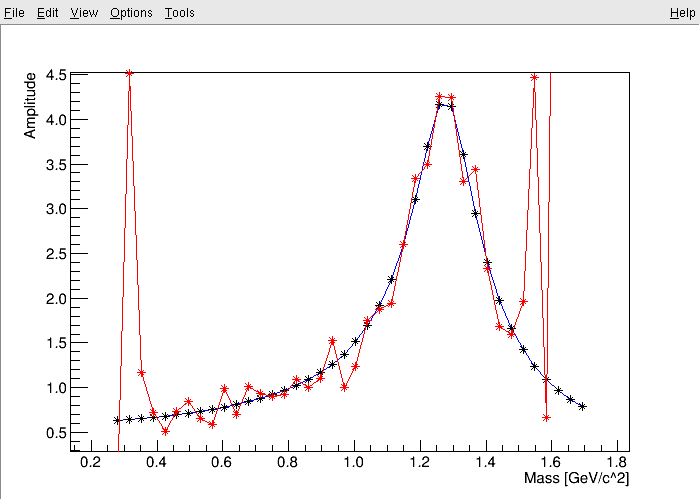
\includegraphics[width=.9\textwidth]{fig/f2_real_time_fit.png}

        \caption{Screenshot of the real-time plot of the decay-amplitude magnitude while fitting a \Pfii{} resonance.
                 In blue, with black points, the initial guess for the fit parameters; in red, the fit parameters.
                 In this case, the initial guess for the fit parameters is the value of the \Pfii{} dynamic shape on the low edges of the bins that partition the mass range.}
        \label{fig:rt_par_fit}
    \end{figure}


    Due to the long fit times, I decided to implement a real-time visualization tool for the fit.
    For each \lstinline!FreedWave!, the \lstinline!RTPlotMIFitModel! class will create a pair of plots for the decay-amplitude magnitude and phase.
    Each plot contains two \ROOT{} graphs: the initial guess for the fit parameters, and the values of the fit parameters updated in real time in every fit iteration.
    The figure~\ref{fig:rt_par_fit} shows a screenshot of the magnitude of the \Pfii{} decaying amplitude.
    By means of these plots, the user does not have to wait until the end of the fit just to find out there was some mistake in the model.
    Moreover, I have experienced that this is also a great debugging utility, \eg{}~for spotting mistakes in the utility routines that convert fit parameters into \pac{yap} free amplitudes. 


    \chapter{Conclusions \& outlook}

    \ac{pwa} is a key tool in the studies of hadronic light- and heavy-meson decays.
    This motivates the development of \pac{yap}, a novel \ac{pwa} toolkit written in \cpp[14]{} with no dependencies besides the \ac{stl}.
    \pac{yap} aims to be physically correct, being extensively tested via a test suite that covers about \SI{90}{\percent} of the code;
    user friendly, with a structure that closely mimics the \ac{pwa} formalism and highlights the physics of the decays;
    computationally efficient, through its smart-caching feature and built-in parallelization support;
    and modular, to be easily coupled to other utilities such as samplers or user interfaces.


    So far, many \acp{pwa} exploited the isobar model, which assumes that the decay proceeds through intermediate two-body decays involving well-defined resonances.
    Therefore, the quality of the decay model depends on the assumption about the resonant content of each partial wave, and on our knowledge of the properties of the resonances themselves (\eg~mass, width, dynamic shape), which comes from past experiments.
    Due to the availability of larger and larger experimental data sets, the systematic effects introduced by these limitations cannot be neglected anymore and an extension of the isobar model is required to improve the \acp{pwa}.
    One possible extension of the isobar model is the model-independent \ac{pwa}, in which the properties of the isobars are directly extracted from the data.

    
    Here, I presented the \pac{yap}-based model-independent fit utility I implemented.
    It allows to perform fits using the amplitude and phase motion as fit parameters; and to simultaneously free multiple waves.


    I tested the utility by fitting several \ac{mc} data sets of $\PDplus\to\Ppiplus\Ppiminus\Ppiplus$ decays with increasingly richer resonant content.
    Because of the complete freedom of the dynamic shape in the model-independent formalism, some ambiguities arise which do not always allow to properly reconstruct the wave content when more than one wave is freed.
    In this case, the knowledge of the zero modes and a two-step fit are needed to extract the wave content from the data.
    With one freed wave and with multiple freed waves without zero modes, the fit utility can already precisely extract the wave content from the data.
    The data generated with the model-independent formalism whose free amplitudes are fixed to the fitted ones always reproduce the source data of the fit.


    The tests show that \pac{yap} is suited to perform model-independent \acp{pwa}.
    A generalization of this fit utility, which also handles mixed-formalism \ac{pwa} and zero modes will be included in \pac{yap}.



%----------------------------------------------------------------------------------------
% BACKMATTER
%
\backmatter
    % Acronyms
    \printnoidxglossaries

    % List of figures
    \cleardoublepage
    \phantomsection
    \pdfbookmark[0]{\listfigurename}{chap:lof}
    \listoffigures

    % Index
    \cleardoublepage
    \phantomsection
    \addcontentsline{toc}{chapter}{\indexname}
    \printindex

    % Bibliography
    \cleardoublepage
    \phantomsection
    \addcontentsline{toc}{chapter}{\bibname}
    \nocite{*}
    \printbibliography

\end{document}
